% Edited, human-readable edition of docs/cavity_concept.md. Every number is taken from that report
% or from the results files it cites; tables marked "generated" come from
% scripts/cavity_report_tables.py. Build: bash docs/report/build.sh
\documentclass[11pt]{article}
% Shared preamble of docs/report/*.tex (single-column article, A4, 11 pt).
\usepackage[T1]{fontenc}
\usepackage[utf8]{inputenc}
\usepackage{lmodern}
\usepackage{microtype}
\usepackage[a4paper,margin=25mm]{geometry}
\usepackage{amsmath,amssymb}
\usepackage{upgreek}
\usepackage[per-mode=symbol]{siunitx}
\usepackage{longtable,booktabs,array,tabularx,multirow,makecell}
\usepackage{calc}
\usepackage{etoolbox}
\usepackage{graphicx}
\graphicspath{{../../results/}}
\usepackage{float}
\usepackage[font=small,labelfont=bf]{caption}
\usepackage{xcolor}
\usepackage[numbers,sort&compress]{natbib}
\usepackage{xurl}
\usepackage[hidelinks]{hyperref}

% Images: scale down to the text width if needed (as in pandoc's template).
\makeatletter
\def\maxwidth{\ifdim\Gin@nat@width>\linewidth\linewidth\else\Gin@nat@width\fi}
\def\maxheight{\ifdim\Gin@nat@height>\textheight\textheight\else\Gin@nat@height\fi}
\makeatother
\setkeys{Gin}{width=\maxwidth,height=\maxheight,keepaspectratio}

% Pandoc output helpers (faithful edition).
\providecommand{\tightlist}{\setlength{\itemsep}{0pt}\setlength{\parskip}{0pt}}
\makeatletter
\patchcmd\longtable{\par}{\if@noskipsec\mbox{}\fi\par}{}{}
\makeatother
\AtBeginEnvironment{longtable}{\footnotesize}
\AtBeginEnvironment{tabularx}{\footnotesize}

% Notation.
\newcommand{\placeholder}[1]{{\color{red!55!black}\ttfamily\small #1}}
\newcommand{\rtHz}{\ensuremath{/\sqrt{\mathrm{Hz}}}}
\DeclareSIUnit\dBc{dBc}
\DeclareSIUnit\ppm{ppm}
\sisetup{range-phrase={\text{ to }},range-units=single,list-units=single}
\setlength{\parskip}{0.4ex}


\title{A cavity-enhanced large-period optical lattice with graded-phase modes\\
for $10^{5}$ to $10^{6}$ cesium atoms}
\author{Rahul Sawant\\\placeholder{[CONFIRM?: co-authors and affiliation]}}
\date{Technical report, \today}

\begin{document}
\maketitle

\begin{abstract}
Static meta-optic tweezer arrays for $10^{6}$ cesium atoms need about \SI{1.4}{\kilo\watt} of
trapping light at \SI{1075}{\nano\metre}, which makes laser power, heat in the metasurface and
damage by absorbing defects the limits on scaling. We show that a build-up cavity cannot reduce the
power of such an array tenfold, because every intracavity focusing element is passed at least twice
per round trip; the enhancement is bounded at 3.2. We then design a cavity-enhanced lattice with a
\SI{4}{\micro\metre} pitch, in which each axis is a self-intersecting ring whose flat-top sheet mode
is set by two graded-phase mirrors and made non-degenerate by a $0.2\times$ intracavity telescope.
Fox--Li simulations of the ring give a barrier depth uniform to \SI{0.23}{\percent} rms over
$10^{6}$ sites, and the three rings need \SI{3.5}{\watt} of input at an enhancement of 300
(\SI{0.69}{\watt} at 1500), against \SI{1.04}{\kilo\watt} for the same lattice in free space.
Mirror figure errors of $\lambda/1000$ rms on every mirror give 2.0 to \SI{4.8}{\percent} before
correction; feedback on depths measured with the atoms restores 0.22 to \SI{0.54}{\percent} in four of
six runs. The constraints move to mirror figure, alignment stability, surface cleanliness at 4.5 to
\SI{48}{\kilo\watt\per\centi\metre\squared} (up to \SI{55}{\kilo\watt\per\centi\metre\squared} on the
vertical ring, which needs its own vertical telescope and sapphire mirrors), and mirror vibration below \SI{0.32}{\pico\metre}\rtHz{} at the
\SI{20}{\kilo\hertz} trap frequency. The same models at $10^{4}$ and $10^{5}$ sites show that the step to
$10^{6}$ is the large one: below it a plain ring without telescope is non-degenerate, needs \SI{0.5}{\watt}
or less, and keeps its in-plane mirrors at \SI{4.2}{\kilo\watt\per\centi\metre\squared}.
\end{abstract}

\tableofcontents

%======================================================================
\section{Introduction}
\label{sec:intro}

A neutral-atom array of $10^{5}$ to $10^{6}$ sites, trapped by meta-optic tweezers, needs trapping
light in proportion to the number of sites. With the meta-hologram of this project (\SI{143}{\milli\kelvin}
site per watt) a \SI{0.2}{\milli\kelvin} trap at every one of $10^{6}$ sites needs \SI{1.40}{\kilo\watt}
at the optics input, and the lenslet array \SI{2.50}{\kilo\watt}. At this power three limits act
together: (i) the laser power itself; (ii) the heat deposited in the metasurface and its substrate;
and (iii) damage, and thermal lensing, caused by absorbing defects on surfaces that carry the full
beam. A build-up cavity is the standard way to reduce the input power, because the light is reused
many times. The question we address is whether a combination of a cavity and meta-optics can reduce
the power by an order of magnitude at $10^{6}$ sites, and which design and simulations support it.

Two experiments are the closest precedents. Park et al.\ built a two-cavity Sr lattice with finesse
5025 and a power enhancement of 1132 at \SI{914}{\nano\metre}, with \SI{489}{\micro\metre} waists and
about \SI{92}{\watt} circulating in a monolithic ULE assembly in vacuum~\cite{Park2022}. Norcia et al.\
imaged 1225 Yb sites in two self-intersecting cavities (finesse 2900 and 3000, waists 268 and
\SI{183}{\micro\metre}) with roughly two orders of magnitude less power than tweezers and at most
\SI{50}{\ppm} loss per mirror~\cite{Norcia2024}. Both used Gaussian modes over arrays of 0.1 to
\SI{1}{\milli\metre}. Neither shaped a flat mode over several millimetres, and neither addressed the
near-degeneracy of the transverse modes that such a mode brings.

In this work, we (i) bound the enhancement of a tweezer array placed inside a cavity
(Section~\ref{sec:tweezer}); (ii) design a three-axis lattice of self-intersecting rings with
graded-phase mirrors and an intracavity telescope, and fit it around the atoms with room for the
imaging objective, a MOT and further beams (Sections~\ref{sec:architecture} and~\ref{sec:access});
(iii) give its power and loss budget (Section~\ref{sec:budget}); (iv) simulate its flat-top mode,
tolerances and correction with a Fox--Li model (Sections~\ref{sec:foxli} and~\ref{sec:correction});
(v) evaluate the intensities, defect limits and thermal deformation on the mirrors
and the heat load and cooling needs (Section~\ref{sec:defects}); (vi) derive the noise requirements set by heating
(Section~\ref{sec:noise}); and (vii) repeat the analysis at $10^{4}$ and $10^{5}$ sites to see which
constraints are specific to $10^{6}$ (Section~\ref{sec:scaling}). Section~\ref{sec:discussion} separates what is shown from what depends
on the model, and lists the next steps. A parameter summary, the commands that reproduce every
result, and the provenance of every number are given in the appendices.

%======================================================================
\section{Why the tweezer array cannot be cavity-enhanced tenfold}
\label{sec:tweezer}

A ring cavity with input transmission $T$ and all other round-trip losses $L$ has the on-resonance
power enhancement
\begin{equation}
  G = \frac{T}{(1-r)^{2}}, \qquad r = \sqrt{(1-T)(1-L)},
  \label{eq:G}
\end{equation}
with the maximum $G_\mathrm{max} = 1/L$ at $T = L$. Here, $G$ is the ratio of circulating to input
power. For $G = 10$ the round-trip loss must stay below \SI{10}{\percent}. An NA 0.5 tweezer array
is not an eigenmode of a pair of mirrors, so the focusing optic must sit inside the cavity, and it
is passed at least twice per round trip. Table~\ref{tab:tweezer} gives the resulting bounds.

\begin{table}[htbp]
\centering
\caption{Largest enhancement of a cavity that contains the focusing optic of a tweezer array.
Efficiencies of the meta-optics from this project's simulations; the refractive and relay values
are assumptions.}
\label{tab:tweezer}
\small
\begin{tabular}{@{}lcc@{}}
\toprule
Intracavity focusing element & Passes per round trip & $G_\mathrm{max}$ \\
\midrule
Meta-hologram, efficiency 0.83 & 2 & 3.2 \\
Pair of meta-objectives, 0.80 each & 4 & 1.7 \\
Pair of refractive objectives, 0.95 each \placeholder{[VALUE?]} & 4 & 5.4 \\
Ideal AR relay, 0.995 per pass \placeholder{[VALUE?]} & 4 & 50 \\
\bottomrule
\end{tabular}
\end{table}

Only the last line reaches 10, and it is not a meta-optic. A degenerate concentric cavity avoids
intracavity lenses: two spherical mirrors share their centre at the atoms and image every focus onto
itself. However, a ray trace of one reflection (NA 0.5, mirror radius 30 or \SI{50}{\milli\metre},
piston, tilt and focus removed) gives a round-trip wavefront error of 0.031 or 0.019 waves rms at a
\SI{100}{\micro\metre} field, 0.28 or 0.17 at \SI{300}{\micro\metre}, and 3.1 or 1.9 at
\SI{1}{\milli\metre}. Each site must stay within a fraction of the linewidth $2\pi/F$, so the finesse
$F$ is limited to 3 to 5 at \SI{100}{\micro\metre} and below 1 at \SI{300}{\micro\metre}. The mirrors
would also fill both NA 0.5 cones that imaging needs. Retro-reflecting the tweezer light through a
second objective onto a mirror gives at most $(1+\sqrt{\eta_\mathrm{return}})^{2}$, i.e.\ 3.2 for the
meta-objective ($\eta_\mathrm{return} = 0.8^{2}\times 0.99$) and 3.8 for a refractive one, and it
forms a $\lambda/2$ axial standing wave in every trap.

Thus the order-of-magnitude saving must come from a different trap geometry: one in which each
photon serves many sites, because each lattice beam crosses every row of the array, and whose mode
can be supported by mirrors alone.

%======================================================================
\section{Architecture}
\label{sec:architecture}

\subsection{Three self-intersecting rings}

The lattice is formed by three build-up cavities, one per axis, mutually detuned by at least
\SI{100}{\mega\hertz} so that their interference averages out (\SI{0.36}{\ppm} of the laser
frequency; the resulting site shift is \SI{0.7}{\nano\metre} at the array edge). Each in-plane axis
is a self-intersecting ring. Its mode crosses the atom plane twice, on arms A and B, at a full angle
$2\theta$ with
\begin{equation}
  \sin\theta = \frac{\lambda}{2a},
  \label{eq:period}
\end{equation}
so that $\theta = \ang{7.72}$ for a period $a = \SI{4}{\micro\metre}$ at $\lambda = \SI{1075}{\nano\metre}$.
Both crossing beams travel in the same direction, so the only fringe period is $a$; a standing-wave
cavity would add $\lambda/2$ fringes along the beams. The two beams of one axis are the same
circulating mode, so their relative phase needs no separate lock. The polarisation is vertical,
perpendicular to the crossing plane, which gives full contrast.\footnote{Horizontal polarisation
would allow Brewster-angle windows, at a contrast $\cos 2\theta = 0.964$.} The $y$-lattice ring has
its arms along $x$, and the $x$-lattice ring is the same ring rotated by \ang{90}.

The mode is a sheet. In the plane it is a super-Gaussian flat-top with amplitude
$\exp(-|u/w|^{20})$, whose intensity is at least 0.99 of the flat level over the array's transverse
range $|u| \le (S/2)(\cos\theta + \sin\theta) = \SI{2.25}{\milli\metre}$. Here, $u$ is the transverse
coordinate of the beam and $S = \SI{4.0}{\milli\metre}$ the side of a $1000 \times 1000$ array. This
gives $w = \SI{2.93}{\milli\metre}$ and an equivalent width $W_\mathrm{eq} = \SI{5.51}{\milli\metre}$.
Vertically the sheet is Gaussian with a \SI{75}{\micro\metre} half-thickness $w_z$ at the crossing,
whose Rayleigh range of \SI{16.4}{\milli\metre} keeps the depth roll-off along the beams within
\SI{1}{\percent} over the array.

\subsection{Graded-phase mirrors and the telescope}

Each half trip, from the crossing on arm A back to the crossing on arm B, is symmetric about a
graded-phase mirror G. With the target flat-top $F$ at the crossing, the mirror phase
\begin{equation}
  \phi_G = -2 \arg(K F)
  \label{eq:graded}
\end{equation}
returns the conjugate field $(KF)^{*}$, and the symmetric return path then gives $F^{*} = F$. Here,
$K$ is the propagation operator from the crossing to G. Hence $F$ is an exact eigenmode of any
lossless symmetric half trip; this is the graded-phase resonator of B\'elanger and
Par\'e~\cite{Belanger1991}. Section~\ref{sec:foxli} shows that a plain ring of this kind is nearly
degenerate. The adopted design therefore puts a $0.2\times$ Keplerian telescope of cylindrical
mirrors in each half trip: a primary P1 ($f = \SI{100}{\milli\metre}$), a secondary P2
($f = \SI{20}{\milli\metre}$) \SI{120}{\milli\metre} further, and G \SI{100}{\milli\metre} beyond P2.
In the layout of Fig.~\ref{fig:layout} the primary is \SI{70}{\milli\metre} from the crossing,
because at \SI{50}{\milli\metre} the mirrors of the two in-plane rings overlap by \SI{4.2}{\milli\metre}.
The ring then has \SI{290}{\milli\metre} from the crossing to G (a quarter of the round trip), a round trip of \SI{1.16}{\metre}, a free
spectral range of \SI{258}{\mega\hertz}, 10 reflections per round trip, and angles of incidence of
\ang{15} (P1), \ang{44} (P2) and \ang{24} (G). In the Fox--Li model it is equivalent to the
\SI{50}{\milli\metre} ring used for most of Sections~\ref{sec:foxli} and~\ref{sec:correction}: depth
uniform to \SI{0.23}{\percent} rms, fundamental loss $1.6\times10^{-8}$ per round trip, nearest
competing mode at $3.3\times10^{-3}$ loss (against $1.1\times10^{-2}$ at \SI{50}{\milli\metre}), and
$\lambda/1000$ errors on all ten mirrors give 2.0 and \SI{4.0}{\percent} uncorrected and 0.42 and
\SI{0.75}{\percent} after six rounds of atom feedback.

The vertical Gaussian is set by a vertical focal length on P1 and a vertical radius on G. For the
\SI{70}{\milli\metre} ring, \SI{40}{\milli\metre} and \SI{143}{\milli\metre} give the
\SI{75}{\micro\metre} waist with a half-trip stability parameter $m = -0.24$, a transverse-mode spacing
of \SI{2.6}{\radian} per round trip (0.42 of a free spectral range), beam half-heights of
\SI{0.33}{\milli\metre} on P1, \SI{0.18}{\milli\metre} on P2 and \SI{0.55}{\milli\metre} on G, and a
\SI{0.32}{\percent} waist change per \SI{0.1}{\percent} radius error. P2 has no vertical power and lies
close to the vertical waist (\SI{88}{\micro\metre}, \SI{81}{\milli\metre} behind P1), which makes it the
hottest in-plane mirror (Section~\ref{sec:defects}).

\begin{figure}[p]
\centering
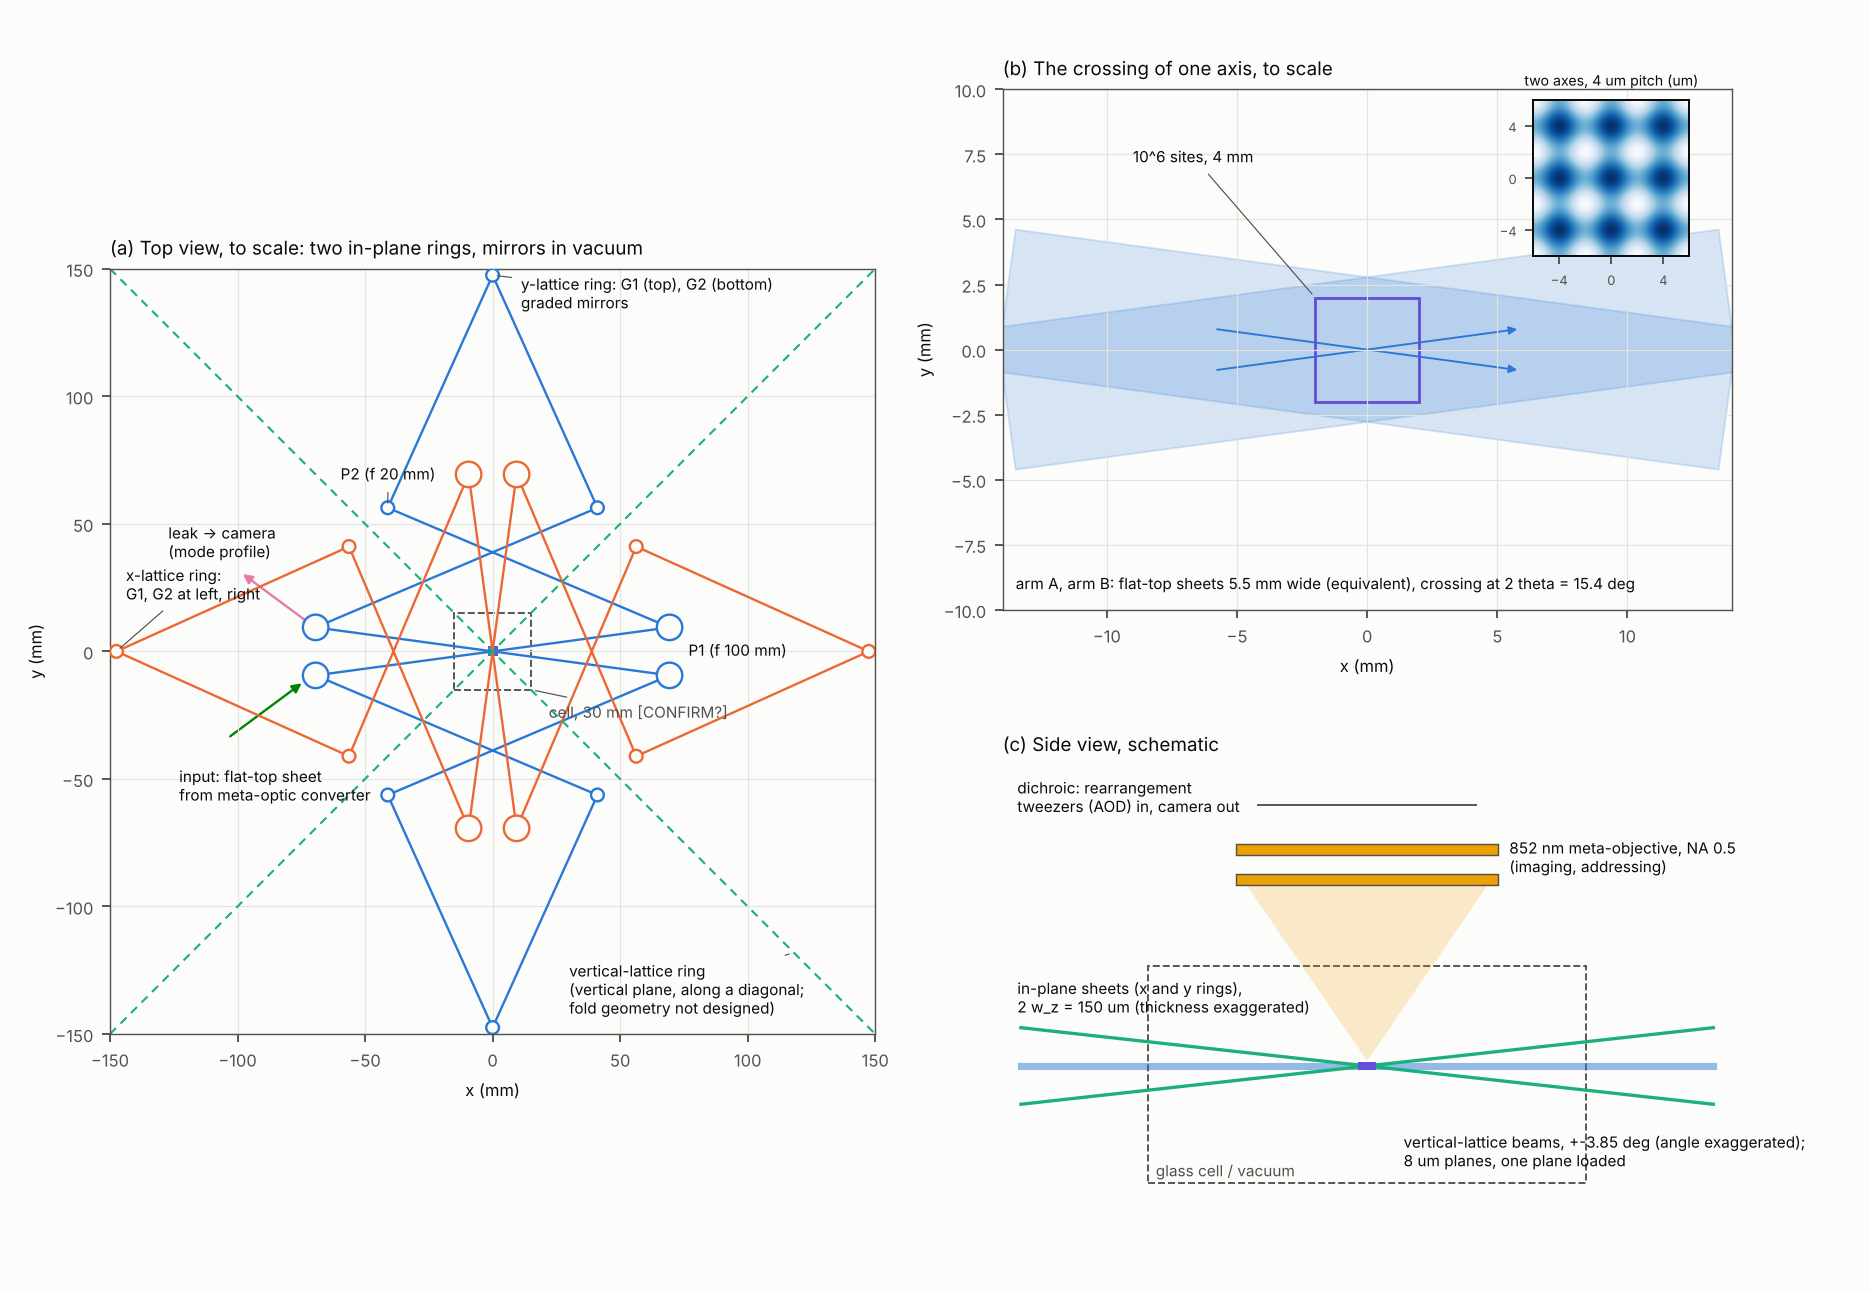
\includegraphics[width=\linewidth]{cavity_layout/sketch_layout.png}
\caption{Arrangement of the in-plane rings. (a) Top view to scale: the $y$-lattice ring (blue) and
the $x$-lattice ring (orange), each a self-intersecting ring with a $0.2\times$ cylindrical telescope
(primary P1, $f = \SI{100}{\milli\metre}$, \SI{70}{\milli\metre} from the crossing; secondary P2,
$f = \SI{20}{\milli\metre}$) and two graded mirrors G1, G2; circles are the mirror apertures (10 and
\SI{5}{\milli\metre}). Dashed diagonals: the corridor for the vertical-lattice ring, whose fold
geometry is shown in Fig.~\ref{fig:vertical} (this sketch predates it). Green: the flat-top input
sheet from an extracavity meta-optic converter; pink: the light leaked by a fold mirror to the mode
camera. (b) The crossing of one axis to scale: the two flat-top sheets (equivalent width
\SI{5.5}{\milli\metre}, $2\theta = \ang{15.4}$) cover the \SI{4}{\milli\metre} array; inset, the
computed intensity of the two incoherent in-plane axes (plane waves, \SI{4}{\micro\metre} pitch).
(c) Side view, schematic, not to scale: the in-plane sheets, the two vertical-lattice beams
($\pm\ang{3.85}$, \SI{8}{\micro\metre} planes) and the \SI{852}{\nano\metre} NA 0.5 meta-objective
above the cell.}
\label{fig:layout}
\end{figure}

\begin{figure}[p]
\centering
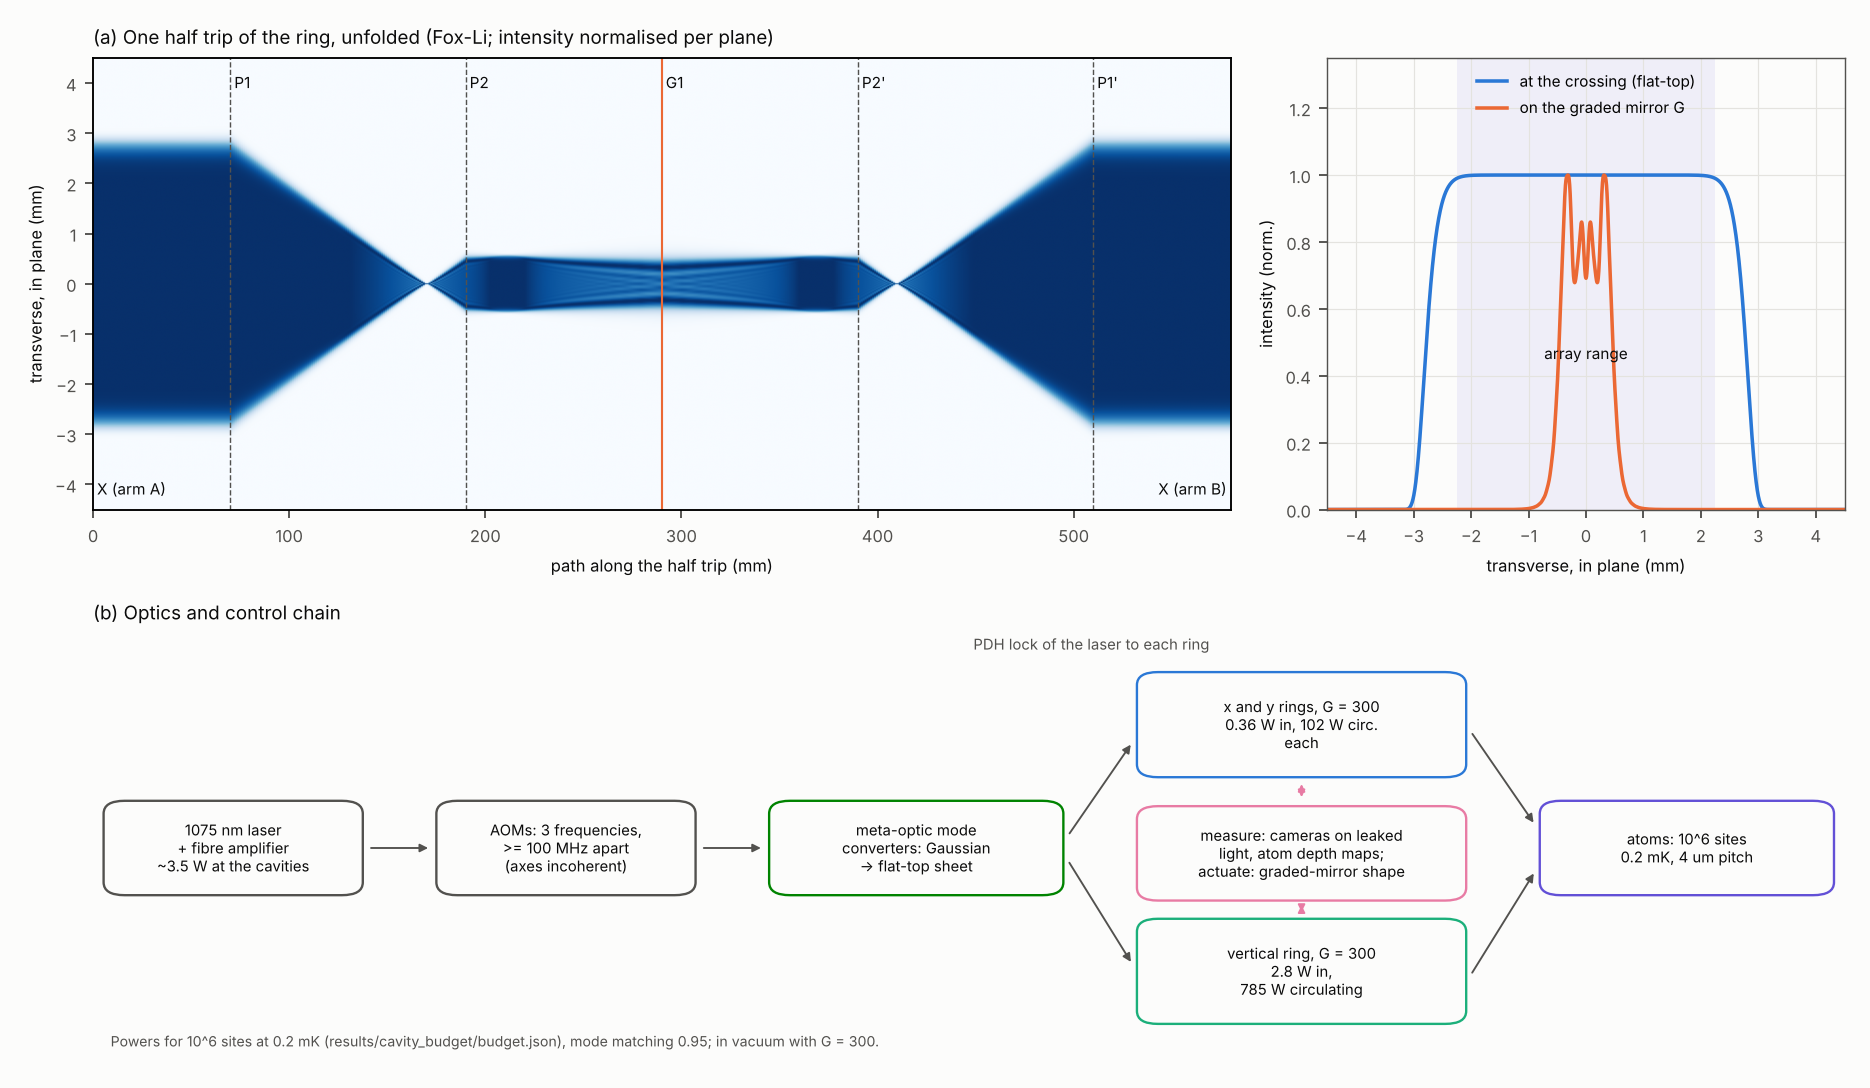
\includegraphics[width=\linewidth]{cavity_layout/sketch_ring.png}
\caption{(a) The beam along one unfolded half trip of the \SI{70}{\milli\metre} ring, from the
crossing on arm A through P1, P2, G1, P2$'$, P1$'$ to the crossing on arm B (Fox--Li, 8192 points;
intensity normalised in each plane). The flat-top is compressed fivefold by the telescope, passes a
line focus between P1 and P2, and is shaped back by G1. Right: the profiles at the crossing and on G.
(b) Optics and control chain for $10^{6}$ sites at \SI{0.2}{\milli\kelvin} with $G = 300$ and mode
matching 0.95: \SI{0.36}{\watt} into each in-plane ring (\SI{102}{\watt} circulating) and
\SI{2.8}{\watt} into the vertical ring (\SI{785}{\watt} circulating). The graded-mirror correction of
Section~\ref{sec:correction} closes the loop from the mode cameras and the atom depth maps.}
\label{fig:ring}
\end{figure}

\subsection{Vertical confinement and the vertical ring}

The in-plane sheets alone give only \SI{0.7}{\kilo\hertz} vertically (Gaussian profile of
\SI{75}{\micro\metre}, \SI{0.4}{\milli\kelvin} at the site). A third ring therefore crosses at
$2\theta_z$ in a vertical plane (period \SI{8}{\micro\metre}, $\theta_z = \ang{3.85}$) and propagates
along the array diagonal. Its beams walk off vertically by $\pm\SI{0.19}{\milli\metre}$ across the
array, so they must be flat-topped vertically as well: \SI{6.9}{\milli\metre} wide, with an equivalent
height of \SI{0.57}{\milli\metre} and an order-10 edge, because an order-20 edge has a
$4\times10^{-4}$ design loss at this small size. This axis takes \SI{785}{\watt} of the
\SI{989}{\watt} circulating at $10^{6}$ sites and \SI{0.2}{\milli\kelvin}.

The vertical ring (Fig.~\ref{fig:vertical}) is planar, in the vertical plane through the atoms that
contains the array diagonal. A planar ring has no image or polarisation rotation, so the flat-top axis
and the polarisation stay horizontal, perpendicular to the ring plane, and the cylindrical telescope
mirrors curve perpendicular to their plane of incidence, where a parabolic cylinder is an exact
cylindrical lens of focal length $R/(2\cos\mathrm{AOI})$. Both half trips fold below the atom plane:
nothing of the ring rises above \SI{9.4}{\milli\metre}, which leaves the space above the atoms to the
objective. Because the crossing half-angle is small, the exit mirrors of the two half trips sit close
together (P1 and P3, \SI{14.8}{\milli\metre} apart vertically at \SI{110}{\milli\metre}), and with an
angle of incidence of at most \ang{45} every fold must turn the beam by at least \ang{90}.

Our choice of telescope for this ring is a compromise between two considerations. First, with the in-plane
telescope ($f = \SI{100}{\milli\metre}$, $0.2\times$) the best layouts found needed a
\SI{60}{\milli\metre} graded-mirror distance, which leaves a competing mode \SI{0.07}{\radian} away with $10^{-5}$ loss and
gives 7.7 to \SI{69}{\percent} non-uniformity for $\lambda/1000$ errors (exploratory run). Second, a
longer telescope must still clear the in-plane rings in three dimensions. A search over the primary
focal length, demagnification, distances and fold directions selects a primary of
$f = \SI{160}{\milli\metre}$, a secondary of $f = \SI{24}{\milli\metre}$ ($0.15\times$), the primary
\SI{110}{\milli\metre} from the atoms and G \SI{120}{\milli\metre} behind the secondary:
\SI{414}{\milli\metre} from the crossing to G, round trip \SI{1.66}{\metre}, free spectral range \SI{181}{\mega\hertz}.
Half trip 1 folds back under the atoms (its folded beam passes \SI{30.6}{\milli\metre} from them) to
G1, \SI{158}{\milli\metre} below the atoms; half trip 2 folds down to \SI{190}{\milli\metre} depth and
back up to G2, \SI{104}{\milli\metre} below the atoms. The clearances are \SI{11.4}{\milli\metre}
between mirror faces (for \SI{4}{\milli\metre} strips; Section~\ref{sec:defects} shows that P2, G and the
return mirrors must be taller, which still fits), \SI{11.1}{\milli\metre} between beams and foreign mirrors, and
\SI{37.8}{\milli\metre} and \SI{35.8}{\milli\metre} to the in-plane rings' mirrors and beams; the
angles of incidence are \ang{8} to \ang{45}. The effective propagation behind the telescope,
$L/M^{2} = \SI{5.3}{\metre}$, is twice that of the in-plane rings (\SI{2.5}{\metre}), which partly
compensates the wider beam.

\begin{figure}[htbp]
\centering
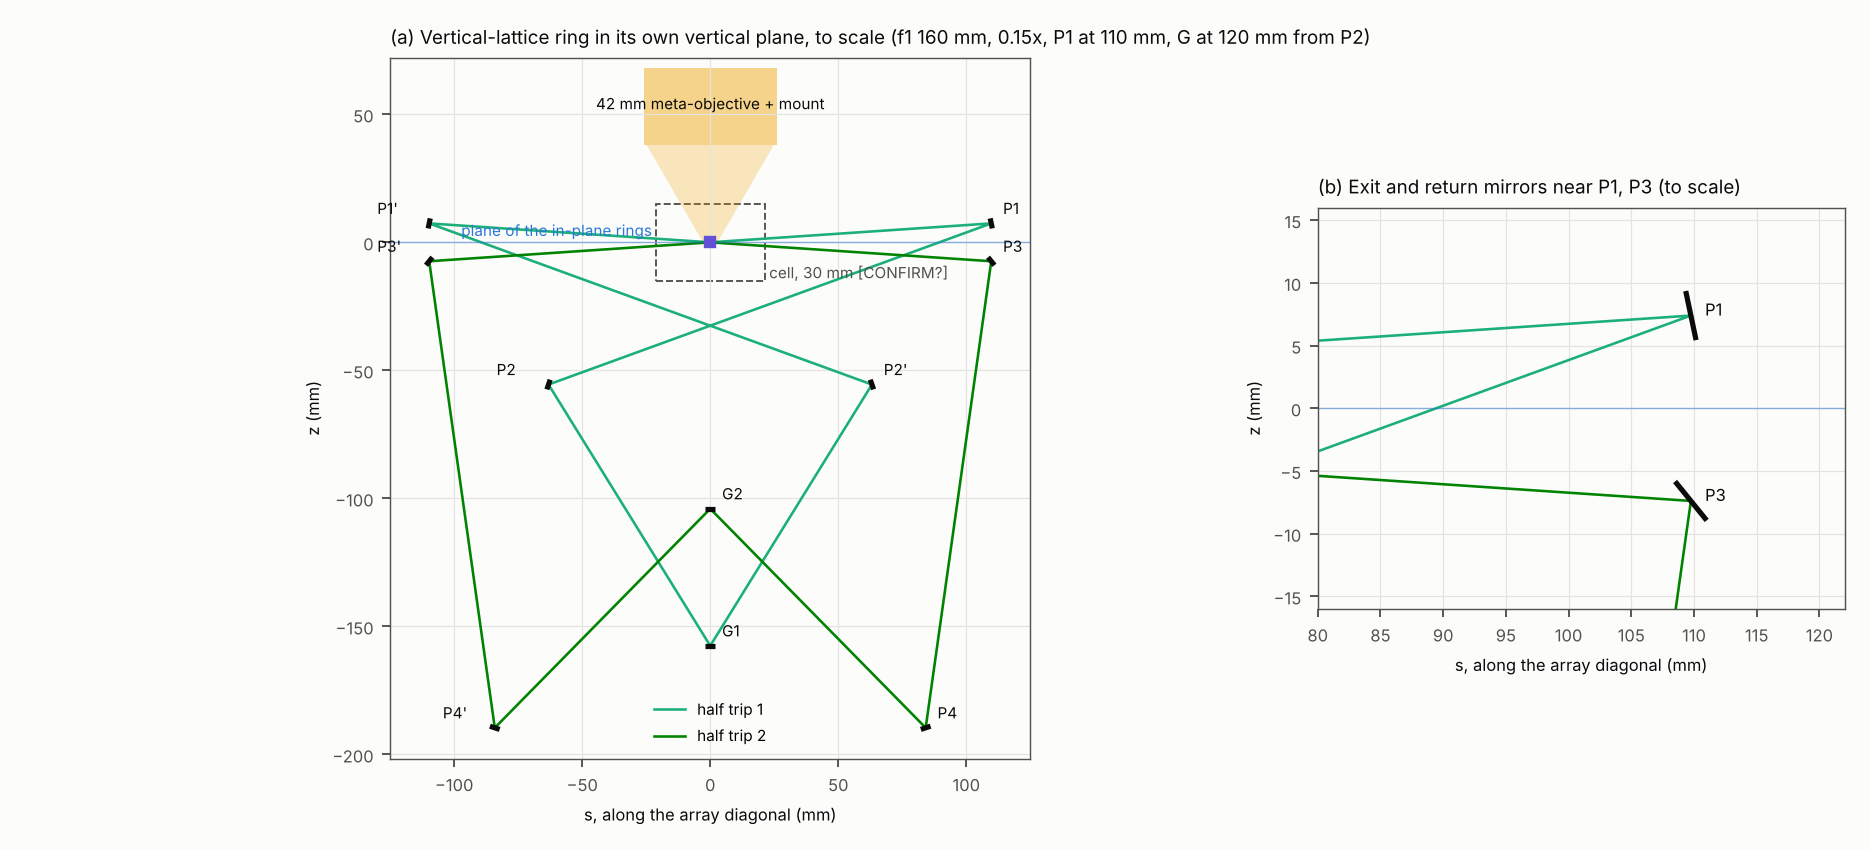
\includegraphics[width=\linewidth]{cavity_layout/sketch_vertical.png}
\caption{The vertical-lattice ring in its vertical plane through the array diagonal, to scale ($s$
along the diagonal, $z$ up). Half trip 1 (light green) leaves the crossing on the upper arm, folds at
P1 back under the atoms to P2, the graded mirror G1 on the vertical axis \SI{158}{\milli\metre} below
the atoms, P2$'$ and P1$'$, and returns on the lower arm; half trip 2 (dark green) folds via P3, P4, G2
(\SI{104}{\milli\metre} below), P4$'$, P3$'$. Black bars: mirror faces (\SI{4}{\milli\metre} strips in
the ring plane as first laid out; the adopted design needs $\pm\SI{2}{\milli\metre}$ on P1, P3 and
$\pm\SI{6}{\milli\metre}$ on the other mirrors, Section~\ref{sec:defects}; widths along the horizontal flat-top axis 12 and \SI{5}{\milli\metre}). Telescope
$f_1 = \SI{160}{\milli\metre}$, $f_2 = \SI{24}{\milli\metre}$. Yellow: the \SI{42}{\milli\metre}
imaging objective with its mount \placeholder{[CONFIRM?]} and the NA 0.5 light cone. (b) The exit and
return mirrors near P1, P3.}
\label{fig:vertical}
\end{figure}

\subsection{Role of the meta-optics}

None of the meta-optics sees the circulating power. They provide (i) the input mode converters, from
a Gaussian to the flat-top sheet; a Gaussian input couples 0.918 of its power into the flat-top mode,
and a flat-top converter is assumed to reach 0.95 \placeholder{[VALUE?]}; (ii) the \SI{852}{\nano\metre}
imaging and addressing objective; and (iii) the tweezers for loading and rearrangement.

%======================================================================
\section{Power and loss budget}
\label{sec:budget}

Each crossing beam needs the peak intensity
\begin{equation}
  I_1 = \frac{U}{4 c \kappa},
  \label{eq:I1}
\end{equation}
where $U$ is the barrier depth and $\kappa = \SI{2.53e-13}{\kelvin}$ per \si{\watt\per\metre\squared}
for Cs at \SI{1075}{\nano\metre} (polarisability 1125 a.u.). For $U = \SI{0.2}{\milli\kelvin}$ this is
\SI{19.8}{\kilo\watt\per\centi\metre\squared}. The circulating power per in-plane axis is
$I_1 W_\mathrm{eq} \sqrt{\pi/2}\, w_z$, independent of the number of beams per axis because one mode
supplies both. Thus the in-plane power scales as the array side, $\sqrt{N}$, against $N$ for tweezers.
The vertical axis scales close to $N$, because its beams must also cover the vertical walk-off
(Table~\ref{tab:power}).

\begin{table}[htbp]
\centering
\caption{Circulating power of the three lattice axes and the input power of hologram tweezers of the
same depth. The hologram column reproduces the \SI{210}{\watt} of the earlier $10^{5}$-site study at
\SI{0.3}{\milli\kelvin}.}
\label{tab:power}
\small
\begin{tabular}{@{}lcccc@{}}
\toprule
$N$, barrier & Per in-plane axis & Vertical axis & Total circulating & Hologram tweezers \\
\midrule
$10^{5}$, \SI{0.2}{\milli\kelvin} & \SI{32}{\watt} & \SI{78}{\watt} & \SI{143}{\watt} & \SI{140}{\watt} \\
$10^{5}$, \SI{0.3}{\milli\kelvin} & \SI{48}{\watt} & \SI{117}{\watt} & \SI{214}{\watt} & \SI{210}{\watt} \\
$10^{6}$, \SI{0.2}{\milli\kelvin} & \SI{102}{\watt} & \SI{785}{\watt} & \SI{989}{\watt} & \SI{1399}{\watt} \\
$10^{6}$, \SI{0.3}{\milli\kelvin} & \SI{154}{\watt} & \SI{1177}{\watt} & \SI{1484}{\watt} & \SI{2098}{\watt} \\
\bottomrule
\end{tabular}
\end{table}

The round-trip loss, with 10 reflections of \SI{50}{\ppm} (the per-mirror bound of
Ref.~\cite{Norcia2024}), and the resulting enhancement are given in Table~\ref{tab:loss}.

\begin{table}[htbp]
\centering
\caption{Round-trip loss and enhancement for the placements considered. The design point is the
over-coupled input coupler $T = 3L$.}
\label{tab:loss}
\small
\begin{tabularx}{\linewidth}{@{}>{\raggedright\arraybackslash}X>{\centering\arraybackslash}p{2.6cm}>{\centering\arraybackslash}p{2.2cm}>{\centering\arraybackslash}p{3.2cm}@{}}
\toprule
Placement & Round-trip loss $L$ & $G_\mathrm{max} = 1/L$ & $G$ at $T = 3L$ (finesse) \\
\midrule
Mirrors in vacuum & $5.0\times10^{-4}$ & 2000 & 1500 (3140) \\
In vacuum, graded mirrors $+10^{-3}$ each & $2.5\times10^{-3}$ & 400 & 300 (627) \\
In vacuum, graded mirrors $+10^{-2}$ each (metasurface) & $2.0\times10^{-2}$ & 49 & 36 (75) \\
Through the cell, 8 AR surfaces at $2.5\times10^{-4}$ \placeholder{[VALUE?]} & $2.5\times10^{-3}$ & 398 & 298 (623) \\
Through the cell, 8 AR surfaces at $10^{-3}$ \placeholder{[VALUE?]} & $8.5\times10^{-3}$ & 118 & 88 (183) \\
Through the cell, 8 Brewster surfaces at $10^{-4}$ \placeholder{[VALUE?]} & $1.3\times10^{-3}$ & 760 & 570 (1192) \\
\bottomrule
\end{tabularx}
\end{table}

We take $T = 3L$ as the design point. It gives 0.75 of the maximum enhancement at half the finesse,
and the enhancement then depends only weakly on the exact loss; Section~\ref{sec:foxli} shows that the
depth tolerances do not depend on the finesse between 47 and 7000. A further reason to stay well below
$G_\mathrm{max}$ is the cavity linewidth: \SI{413}{\kilo\hertz} at $G = 300$ and \SI{82}{\kilo\hertz}
at $G = 1500$ for the \SI{258}{\mega\hertz} free spectral range. The linewidth converts laser frequency
noise into intensity noise, which Norcia et al.\ identify as a heating source (\SI{190}{\milli\second}
time constant)~\cite{Norcia2024}, and Section~\ref{sec:noise} quantifies the cost. We therefore
recommend $G \approx 300$ with mirrors in vacuum, i.e.\ \SI{3.5}{\watt} for $10^{6}$ sites at
\SI{0.2}{\milli\kelvin}, and use $G = 1500$ (\SI{0.69}{\watt}) as the upper bound. At equal radial trap
frequency instead of equal depth (\SI{41}{\kilo\hertz}, which needs a \SI{0.86}{\milli\kelvin} barrier)
the in-vacuum lattice needs \SI{1.4}{\watt} at $G = 1500$ and \SI{6.9}{\watt} through good AR windows.

\begin{figure}[htbp]
\centering
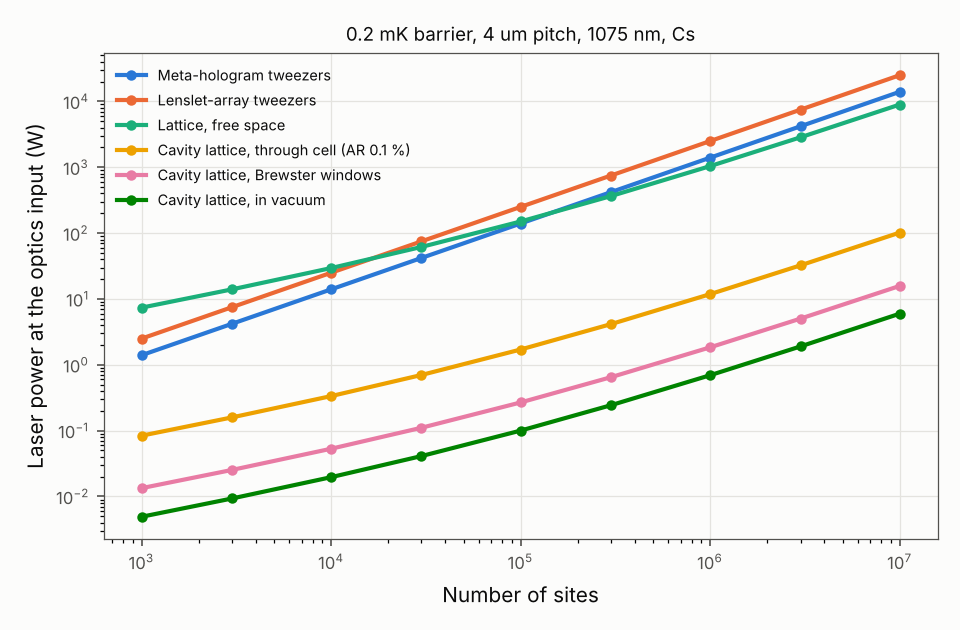
\includegraphics[width=0.85\linewidth]{cavity_budget/power_scaling.png}
\caption{Laser power at the input of the trapping optics versus the number of sites, for a
\SI{0.2}{\milli\kelvin} barrier at \SI{1075}{\nano\metre} and \SI{4}{\micro\metre} pitch. Tweezer
lines: 143 (hologram) and 80 (lenslet) \si{\milli\kelvin} site per watt from earlier simulations of
this project. Lattice lines: two in-plane axes and one vertical axis (\SI{8}{\micro\metre} period),
flat-top times Gaussian sheets ($w_z = \SI{75}{\micro\metre}$), mode matching 0.95; cavity enhancement
for $T = 3L$ with 10 reflections of \SI{50}{\ppm} per round trip, plus 8 AR surfaces of
\SI{0.1}{\percent} (through the cell) or 8 Brewster surfaces of $10^{-4}$.}
\label{fig:power}
\end{figure}

The vertical axis dominates at $10^{6}$ sites. Three options reduce it, none simulated here: (i) a
larger vertical period, since the power scales as $1/a_z$ (as does the vertical trap frequency);
(ii) propagation along an array side instead of the diagonal, at about half the power but with less
clearance to one in-plane ring; and (iii) a lower vertical barrier, if imaging tolerates it. Without
the vertical axis the in-plane lattices need \SI{205}{\watt} circulating at $10^{6}$ sites, i.e.\
\SI{0.7}{\watt} of input at $G = 300$.

%======================================================================
\section{The flat-top cavity mode}
\label{sec:foxli}

\subsection{Method}

We model the horizontal profile with a one-dimensional strip Fox--Li model on 8192 points over
\SI{24}{\milli\metre} (\SI{2.9}{\micro\metre} sampling), with exact scalar angular-spectrum
propagation, hard apertures at every mirror and the graded-phase design computed through the actual
elements. The vertical profile is separable; a separable two-dimensional propagation agrees with the
product of one-dimensional propagations to $2\times10^{-3}$. The driven steady state
$(I - r e^{i\psi} R)E = t E_\mathrm{in}$ is solved by GMRES. Here, $R$ is the round-trip operator,
$\psi$ the round-trip phase set by the laser, and $E_\mathrm{in}$ the input field. The laser is locked
to the $\psi$ of maximum circulating power, found by re-centring on the round-trip phase of the
circulating field followed by a golden-section search. The fields of the two arms are propagated
across the array, combined with the vertical Gaussian (width and Gouy phase) and sampled at
$101 \times 101$ sites spanning the $10^{6}$-site array. The metrics are the rms and minimum-to-mean
ratio of the barrier depth, and the site displacement along the fringe normal with and without its
affine part (a uniform pitch change or rotation is a calibration, not an error). Unless stated, the
input is the target flat-top, $G = 300$ and the lumped loss is $3\times10^{-4}$. The model reproduces
the strip Gaussian mode of a plane-concave design and its first-order Gouy phase to $10^{-4}$, and the
driven enhancement against Eq.~\eqref{eq:G} to $10^{-4}$. The results do not change between 4096,
8192 and 16384 points (depth rms 0.23148, 0.23149 and \SI{0.23149}{\percent}).

\subsection{Ideal designs and the degeneracy of the plain ring}

Every design reproduces the target. Over $10^{6}$ sites the barrier depth is uniform to
\SI{0.23}{\percent} rms (minimum over mean 0.990, set by the \SI{1}{\percent} design tolerance at the
flat edge). The site displacement is \SI{6}{\nano\metre} rms, all of it affine (residual
\SI{0.03}{\nano\metre}), and it comes from the differential Gouy phase of the two sheets.
Table~\ref{tab:designs} compares the designs.

\begin{table}[htbp]
\centering
\caption{Ideal designs. Spectra by full diagonalisation of the round trip on 4096 points. The graded
mirror column gives its peak-to-valley phase and maximum deflection angle.}
\label{tab:designs}
\small
\begin{tabularx}{\linewidth}{@{}>{\raggedright\arraybackslash}p{3.6cm}>{\centering\arraybackslash}X>{\centering\arraybackslash}X>{\centering\arraybackslash}p{3.4cm}>{\centering\arraybackslash}X@{}}
\toprule
Design & Fresnel number $w^{2}/(\lambda p)$ & Fundamental loss per round trip & Nearest competing mode (phase, loss) & Graded mirror PV, deflection \\
\midrule
Plane folds, $p = \SI{150}{\milli\metre}$ & 53 & $8\times10^{-10}$ & \SI{0.017}{\radian}, $2\times10^{-9}$ & \SI{5.9}{\radian}, 0.004 \\
Plane folds, $p = \SI{300}{\milli\metre}$ & 27 & $1\times10^{-9}$ & \SI{0.033}{\radian}, $6\times10^{-8}$ & \SI{9.0}{\radian}, 0.004 \\
Plane folds, $p = \SI{600}{\milli\metre}$ & 13 & $3\times10^{-6}$ & \SI{0.067}{\radian}, $8\times10^{-6}$ & \SI{13}{\radian}, 0.003 \\
Telescope $0.2\times$, Keplerian & -- & $1.4\times10^{-8}$ & all modes lose $\ge 1.1\times10^{-2}$ & \SI{24}{\radian}, 0.013 \\
Telescope $0.1\times$, Keplerian & -- & $2.3\times10^{-8}$ & all modes lose $\ge 1.4\times10^{-2}$ & \SI{36}{\radian}, 0.026 \\
Telescope $0.2\times$, Galilean & -- & $2.6\times10^{-6}$ & \SI{0.33}{\radian}, $1.5\times10^{-3}$ & \SI{30}{\radian}, 0.013 \\
\bottomrule
\end{tabularx}
\end{table}

With plane folds the mode spacing is about $\lambda p / w^{2}$, the inverse Fresnel number of the flat
mode: \SI{0.017}{\radian} at $p = \SI{150}{\milli\metre}$ and \SI{0.067}{\radian} at
\SI{600}{\milli\metre}, with no loss difference. A perturbation of the round-trip phase $\delta\phi$
mixes the nearest mode into the fundamental with an amplitude of about $\delta\phi/0.017$. A
$\lambda/1000$ surface error, i.e.\ \SI{12.6}{\milli\radian} of reflected phase, is then an order-one
admixture. This is the flat-top counterpart of the $w^{4}$ alignment sensitivity of large Gaussian
modes noted by Park et al.~\cite{Park2022}. Curved folds do not help: a single cylindrical fold raised
the spacing to at most \SI{0.025}{\radian}, and Fourier-transform configurations made it smaller
(exploratory runs). A demagnifying telescope of magnification $M$ makes the remaining path $L$ to the
graded mirror act, seen from the crossing, like a path $L/M^{2}$. The mode on G then has a Fresnel
number near 1, the regime of strong mode discrimination of the graded-phase resonator. In the
$0.2\times$ design with the primary at \SI{50}{\milli\metre} every competing mode loses at least
\SI{1.1}{\percent} per round trip, a million times the loss of the fundamental; in the adopted
\SI{70}{\milli\metre} ring the nearest competitor lies \SI{0.216}{\radian} away with $3.3\times10^{-3}$ loss. The edge order is a compromise: orders 10 and 40 give the same
uniformity (0.24 and \SI{0.23}{\percent}) at equivalent widths of 6.78 and \SI{4.98}{\milli\metre},
but in the telescope ring order 40 raises the design loss from $1.4\times10^{-8}$ to $3.4\times10^{-5}$
and brings a competing mode to $4.7\times10^{-3}$ loss, so we keep order 20.

\subsection{Tolerances}

Table~\ref{tab:tolerance} gives the barrier-depth non-uniformity for figure errors, curvature errors
and tilts, as the median over two random realisations and correlation lengths of 0.5 and
\SI{2}{\milli\metre} referred to the crossing. Figure errors are rms surface heights over the beam,
with reflected phase $4\pi h/\lambda$; both graded mirrors are perturbed independently, and tilts and
curvature errors are on one graded mirror. The P1 rows put the same error on the incoming primary of
both half trips; Section~\ref{sec:correction} treats independent errors on all ten mirrors.

\begin{table}[htbp]
\centering
\caption{Barrier-depth non-uniformity over the $10^{6}$-site array (rms, median over realisations)
and, in parentheses, the lowest enhancement relative to the analytic value. K: Keplerian, G:
Galilean. Generated from the Fox--Li results by \texttt{scripts/cavity\_report\_tables.py}.}
\label{tab:tolerance}
% generated by scripts/cavity_report_tables.py; do not edit
\begin{tabularx}{\linewidth}{@{}>{\raggedright\arraybackslash}p{3.6cm}>{\centering\arraybackslash}X>{\centering\arraybackslash}X>{\centering\arraybackslash}X>{\centering\arraybackslash}X>{\centering\arraybackslash}X@{}}
\toprule
Perturbation & Plane folds, 150 mm & Plane folds, 300 mm & Telescope 0.2x K & Telescope 0.1x K & Telescope 0.2x G \\
\midrule
G figure, rms, 0.001 waves & 31 \% (0.61) & 17 \% (0.84) & 2.7 \% (0.97) & 1.3 \% (0.98) & 6 \% (0.94) \\
G figure, rms, 0.003 waves & 49 \% (0.42) & 44 \% (0.41) & 7.6 \% (0.78) & 3.9 \% (0.82) & 18 \% (0.59) \\
G figure, rms, 0.01 waves & 59 \% (0.15) & 57 \% (0.19) & 21 \% (0.36) & 14 \% (0.21) & 24 \% (0.08) \\
P1 figure, rms, 0.001 waves & - & - & 2.4 \% (0.99) & 1.3 \% (0.96) & 8.5 \% (0.90) \\
P1 figure, rms, 0.003 waves & - & - & 7.4 \% (0.90) & 3.9 \% (0.73) & 25 \% (0.41) \\
P1 figure, rms, 0.01 waves & - & - & 26 \% (0.14) & 14 \% (0.09) & 60 \% (0.08) \\
G $x^2$ sag at beam half-width, 0.001 waves & 5.7 \% (1.00) & 2.8 \% (1.00) & 0.82 \% (1.00) & 0.3 \% (1.00) & 0.87 \% (1.00) \\
G $x^2$ sag at beam half-width, 0.003 waves & 18 \% (0.98) & 8.7 \% (1.00) & 2.6 \% (0.98) & 0.65 \% (0.99) & 2.9 \% (0.99) \\
G $x^2$ sag at beam half-width, 0.01 waves & 61 \% (0.86) & 31 \% (0.96) & 12 \% (0.70) & 2 \% (0.90) & 5.5 \% (0.78) \\
G tilt, 0.3~\si{\micro\radian} & 5.7 \% (0.92) & 3.3 \% (0.97) & 0.26 \% (1.00) & 0.23 \% (1.00) & 0.27 \% (1.00) \\
G tilt, 1~\si{\micro\radian} & 15 \% (0.68) & 11 \% (0.83) & 0.43 \% (1.00) & 0.25 \% (1.00) & 0.53 \% (1.00) \\
G tilt, 3~\si{\micro\radian} & 67 \% (0.39) & 26 \% (0.58) & 1.1 \% (1.00) & 0.38 \% (1.00) & 1.4 \% (1.00) \\
G tilt, 10~\si{\micro\radian} & 80 \% (0.26) & 73 \% (0.33) & 3.7 \% (0.97) & 1 \% (0.99) & 5.1 \% (0.96) \\
P1 tilt, 0.3~\si{\micro\radian} & - & - & 1.1 \% (1.00) & 0.6 \% (1.00) & 0.73 \% (1.00) \\
P1 tilt, 1~\si{\micro\radian} & - & - & 3.7 \% (0.97) & 1.9 \% (0.99) & 2.4 \% (0.99) \\
P1 tilt, 3~\si{\micro\radian} & - & - & 11 \% (0.83) & 5.8 \% (0.93) & 8.1 \% (0.91) \\
P1 tilt, 10~\si{\micro\radian} & - & - & 33 \% (0.56) & 20 \% (0.61) & 24 \% (0.59) \\
\bottomrule
\end{tabularx}

\end{table}

Four results follow. (i) The telescope reduces the sensitivity to graded-mirror figure 6 to 11 fold,
and to graded-mirror tilt 20 to 60 fold. (ii) The large telescope mirrors now carry the tightest
tolerances: a $\lambda/1000$ rms figure error on the two incoming primaries gives \SI{2.4}{\percent}
rms, and a \SI{1}{\micro\radian} tilt of both \SI{3.7}{\percent}. (iii) The $0.1\times$ telescope halves
these numbers but doubles the intensity on the small mirrors. (iv) The Galilean form is 2 to 3.5 times
more sensitive to figure errors than the Keplerian at the same magnification, though slightly less
sensitive to primary tilt, because its design loss and its nearest mode are closer to the
fundamental. In addition, the finesse barely matters. With a fixed $\lambda/300$ figure error the
non-uniformity is 5.2 to \SI{5.7}{\percent} at $G = 30$, 100, 300, 1000 and 3000 (finesse 47 to 7159),
because the admixture is set by the mode spacing, not by the linewidth (Fig.~\ref{fig:tolerance}).

\begin{figure}[htbp]
\centering
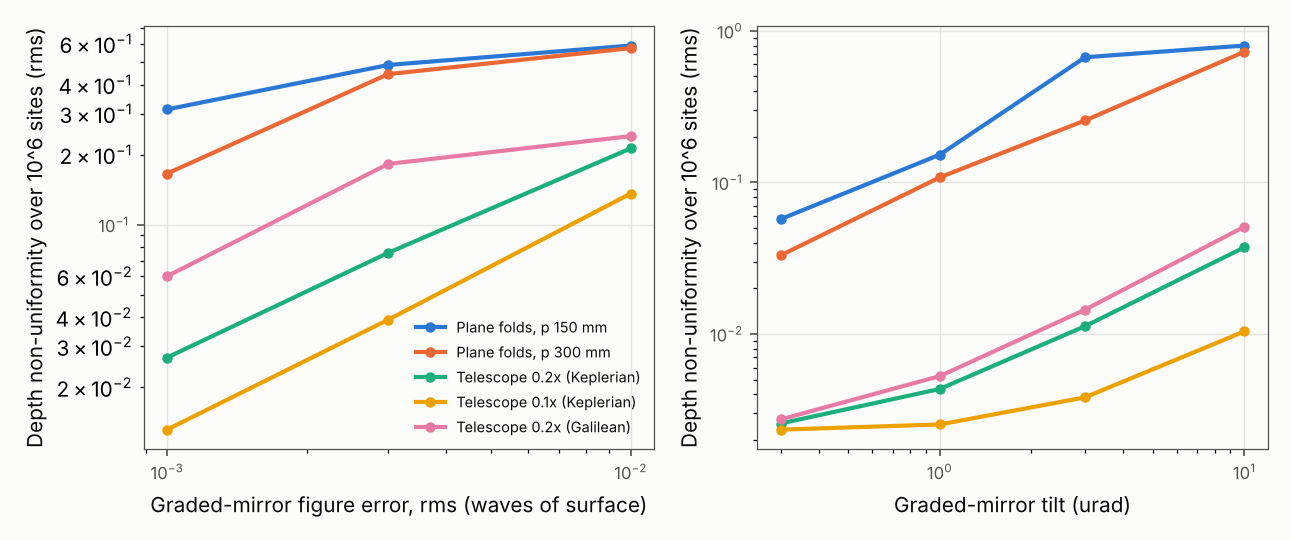
\includegraphics[width=0.9\linewidth]{cavity_foxli/tolerances.png}
\caption{Barrier-depth non-uniformity over the $10^{6}$-site array (rms over $101\times101$ sampled
sites) versus the rms figure error of both graded mirrors (left, median over realisations) and the
tilt of one graded mirror (right), for plane-fold rings of $p = 150$ and \SI{300}{\milli\metre} and for
telescope rings. Fox--Li strip model, 8192 points, $G = 300$, flat-top input,
$w_z = \SI{75}{\micro\metre}$.}
\label{fig:tolerance}
\end{figure}

The cavity filters input mismatch. A flat-top input 2\% too narrow or too wide, or offset by
\SI{100}{\micro\metre}, changes the depth uniformity by at most 0.022 percentage points and the
enhancement by at most \SI{0.6}{\percent}. A Gaussian input with the optimal waist couples 0.918 of
its power and changes the uniformity from 0.23 to \SI{0.42}{\percent} rms. Thus the extracavity mode
converter, the meta-optic role, needs only modest accuracy. Conversely, a ring without graded mirrors
(plane folds and telescope, same flat-top input) gives 12 to \SI{22}{\percent} rms at 0.86 to 0.87 of
the enhancement, because the flat-top is not its eigenmode.

\subsection{Can the graded mirror be a metasurface?}

Quantising $\phi_G$ to 8, 16 or 32 levels gives 19, 12 and \SI{4.5}{\percent} rms, at 0.14, 0.23 and
0.52 of the ideal enhancement. White pixel phase noise of 0.02, 0.05 and \SI{0.1}{\radian} gives 1.5,
3.8 and \SI{7.4}{\percent} rms and reduces the enhancement to 0.89, 0.52 and 0.15 of the ideal. The
SiN libraries of this project at \SI{1075}{\nano\metre} (LPCVD and Si-rich, period 0.45 to
\SI{0.5}{\micro\metre}, height 1.3 to \SI{1.6}{\micro\metre}) give a phase slope of 19 to
\SI{31}{\radian\per\micro\metre} over the $2\pi$ range. Hence \SI{5}{\nano\metre} rms width noise is
0.10 to \SI{0.15}{\radian} in transmission, and about twice that in a reflective double pass (an
estimate; no reflective library was simulated).\footnote{The noise model sets white noise per
\SI{2.9}{\micro\metre} grid cell, so it overstates the mode distortion from \SI{0.5}{\micro\metre}
pixels, whose scatter leaves the cavity at large angles. The loss, about $\sigma^{2}$ per bounce, does
not depend on this.} A metasurface graded mirror therefore needs sub-nanometre width control, or it
must accept $G \approx 36$. The required phase is smooth (\SI{24}{\radian} peak to valley, deflection
at most 0.013), so a continuous freeform surface under an IBS coating is the natural realisation
\placeholder{[REF?: freeform figuring at nm rms over mm apertures]}.

%======================================================================
\section{Correcting the residual non-uniformity}
\label{sec:correction}

\subsection{Method}

The depth map of each axis is the product of the profiles of its two crossing beams, and each graded
mirror shapes one of them, so the residual non-uniformity can be corrected by re-shaping the two
graded mirrors. We put independent smooth figure errors, random tilts or both on every mirror of the
ring: 8 telescope reflections and 2 graded mirrors for the $0.2\times$ ring, and 4 folds and 2 graded
mirrors for the plain \SI{150}{\milli\metre} ring. Correlation lengths are referred to the crossing and
scaled by the beam size on each mirror. We compare three corrections. (i) Open loop: G1 and G2 are
redesigned through the half trips as measured,
\begin{equation}
  \phi = \arg\!\left(K_\mathrm{out}^{\dagger} T_\mathrm{out}\right) - \arg\!\left(K_\mathrm{in} T_\mathrm{in}\right),
  \label{eq:redesign}
\end{equation}
which reduces to Eq.~\eqref{eq:graded} for a symmetric, unperturbed half trip. Here, $K_\mathrm{in}$
and $K_\mathrm{out}$ are the propagations to and from G and $T_\mathrm{in}$, $T_\mathrm{out}$ the
target fields at the crossing. Metrology noise is a smooth random error map of the stated surface rms
on every mirror, plus \SI{0.1}{\micro\radian} of tilt error when tilts are present. (ii) Closed loop
from the atoms, with no knowledge of the errors: each round the barrier depth at $101\times101$
sampled sites is measured with 0 or \SI{1}{\percent} multiplicative noise per site and fitted as
$a(\xi_A)\,b(\xi_B)$ by log-linear least squares with a smoothness penalty. Here, $\xi_A$ and $\xi_B$
are the transverse coordinates of the two beams. The target profiles are multiplied by
$(a,b)^{-1/2}$ and G1, G2 redesigned with the nominal model, for six rounds. (iii) The same loop with
a camera on the light transmitted by a cavity mirror instead of the atoms. Tables~\ref{tab:corr_tel}
and~\ref{tab:corr_plain} give the results.

\begin{table}[htbp]
\centering
\caption{Telescope ring, $0.2\times$: depth rms over the $10^{6}$-site array; two random realisations
where shown, separated by a slash. Camera loop: \SI{10}{\micro\metre} pixels, 48 bins.
Generated by \texttt{scripts/cavity\_report\_tables.py}.}
\label{tab:corr_tel}
{\setlength{\tabcolsep}{2.5pt}% generated by scripts/cavity_report_tables.py; do not edit
\begin{tabularx}{\linewidth}{@{}>{\raggedright\arraybackslash}p{2.6cm}>{\centering\arraybackslash}X>{\centering\arraybackslash}X>{\centering\arraybackslash}X>{\centering\arraybackslash}X>{\centering\arraybackslash}X>{\centering\arraybackslash}X>{\centering\arraybackslash}X>{\centering\arraybackslash}X>{\centering\arraybackslash}X@{}}
\toprule
Errors on every mirror & Uncorrected & Perfect metrology & 0.1 nm metrology & 0.3 nm metrology & 1 nm metrology & Atom loop, 6 rounds & Camera loop, 0.5 \% noise & + 1 \% pixel response & + 1 \% flat field \\
\midrule
$\lambda/1000$ figure, 2 mm & 2 / 4.8 \% & 0.49 / 0.54 \% & 0.68 / 0.61 \% & 1.3 / 1.4 \% & 3.9 / 4.6 \% & 0.48 / 1.9 \% & 0.49 / 1.3 \% & 0.52 / 1.3 \% & 0.61 / 1.3 \% \\
$\lambda/1000$ figure, 0.5 mm & 3.6 \% & 2.4 \% & 2.3 \% & 2.3 \% & 3.9 \% & 2.3 \% & 2.8 \% & 2.8 \% & 3 \% \\
$\lambda/300$ figure, 2 mm & 7.1 / 22 \% & 1.4 / 1.7 \% & 1.5 / 2 \% & 1.9 / 2.9 \% & 4.1 / 7.2 \% & 1.5 / 48 \% & 1.6 / 6.7 \% & 1.6 / 6.8 \% & 1.6 / 6.9 \% \\
tilts, 1~\si{\micro\radian} rms & 1.2 / 1.8 \% & 0.43 / 0.58 \% & 0.53 / 0.48 \% & 1.3 / 1.3 \% & 3.9 / 4.2 \% & 0.22 / 0.23 \% & 0.37 / 0.52 \% & 0.41 / 0.56 \% & 0.51 / 0.63 \% \\
$\lambda/1000$ + 0.3~\si{\micro\radian} tilts & 2.9 \% & 0.6 \% & 0.71 \% & 1.4 \% & 3.9 \% & 0.54 \% & 0.61 \% & 0.64 \% & 0.72 \% \\
\bottomrule
\end{tabularx}
}
\end{table}

\begin{table}[htbp]
\centering
\caption{Plain ring with plane folds, $p = \SI{150}{\milli\metre}$, as Table~\ref{tab:corr_tel}.}
\label{tab:corr_plain}
% generated by scripts/cavity_report_tables.py; do not edit
\begin{tabularx}{\linewidth}{@{}>{\raggedright\arraybackslash}p{2.1cm}>{\centering\arraybackslash}X>{\centering\arraybackslash}X>{\centering\arraybackslash}X>{\centering\arraybackslash}X>{\centering\arraybackslash}X>{\centering\arraybackslash}X@{}}
\toprule
\hspace{0pt}Errors on every mirror & \hspace{0pt}Uncorrected & \hspace{0pt}Perfect metrology & \hspace{0pt}0.1 nm metrology & \hspace{0pt}0.3 nm metrology & \hspace{0pt}1 nm metrology & \hspace{0pt}Atom loop, 6 rounds \\
\midrule
$\lambda/1000$ figure, 2 mm & 20 / 42 \% & 0.23 / 0.23 \% & 0.69 / 2.1 \% & 2.2 / 6.2 \% & 11 / 19 \% & 3.6 / 1.6 \% \\
$\lambda/1000$ figure, 0.5 mm & 24 \% & 0.26 \% & 0.7 \% & 2.2 \% & 11 \% & 0.94 \% \\
$\lambda/300$ figure, 2 mm & 42 / $1.3\times10^{2}$ \% & 0.24 / 0.25 \% & 0.73 / 2 \% & 2.2 / 6.2 \% & 11 / 19 \% & 49 / 37 \% \\
tilts, 1~\si{\micro\radian} rms & 19 / 4.8 \% & 1.9 / 0.32 \% & 3.1 / 1.8 \% & 4.1 / 5.9 \% & 13 / 19 \% & 20 / 0.41 \% \\
$\lambda/1000$ + 0.3~\si{\micro\radian} tilts & 56 \% & 1.9 \% & 3.1 \% & 4.1 \% & 13 \% & 44 \% \\
\bottomrule
\end{tabularx}

\end{table}

\subsection{Open loop and the limits of mirror metrology}

Perfect metrology removes 63 to \SI{92}{\percent} of the non-uniformity of the telescope ring:
$\lambda/1000$ errors on all ten mirrors fall from 2.0 to \SI{4.8}{\percent} to 0.49 to
\SI{0.54}{\percent}, and \SI{1}{\micro\radian} tilts to 0.43 to \SI{0.58}{\percent}. The floor arises
because a phase error on a mirror away from G becomes partly an amplitude error at G and at the
crossing, which a phase-only mirror cannot undo; in a test ring, a redesign through a half trip with an
error on its primary reduced the round-trip infidelity only fourfold, from $1.5\times10^{-3}$ to
$3.2\times10^{-4}$. Errors on a \SI{0.5}{\milli\metre} scale leave 2.3 to \SI{2.4}{\percent}.

The open loop is only as good as the metrology. At \SI{0.1}{\nano\metre} rms per mirror the gain is
kept, \SI{0.3}{\nano\metre} leaves 1.3 to \SI{1.4}{\percent}, and \SI{1}{\nano\metre} (3.9 to
\SI{4.6}{\percent}) is no better than no correction. The best large-optics programmes reach
\SI{0.1}{\nano\metre} to \SI{0.3}{\nano\metre} on the instrument. Advanced LIGO test-mass substrates were
ion-beam figured to 0.08 to \SI{0.23}{\nano\metre} rms over the central \SI{160}{\milli\metre}
(specification below \SI{0.3}{\nano\metre}, power and astigmatism removed)~\cite{LIGO2015,LIGOE080512},
and the metrology interferometer was specified for a repeatability below \SI{0.15}{\nano\metre} rms,
with \SI{0.1}{\nano\metre} as the goal~\cite{LIGOE080508}. EUV projection mirrors were measured with
\SI{27}{\pico\metre} rms repeatability and \SI{46}{\pico\metre} reproducibility, and one mirror reached
\SI{0.10}{\nano\metre} rms figure~\cite{Kurz2004}. However, three differences make our requirement
harder. First, it is absolute, per mirror, and must hold after coating; coating raised the LIGO end
test mass from 0.18 to \SI{0.69}{\nano\metre} rms and the input test mass from 0.15 to
\SI{0.31}{\nano\metre}~\cite{LIGO2015}, more than our whole tolerance. Repeatability is not absolute
accuracy, and independent absolute calibrations of reference flats agree only to
\placeholder{[VALUE?: approx. 0.4 nm rms, verify]}. Second, our mirrors are off-axis cylindrical or
freeform surfaces used at \ang{15} to \ang{38} incidence, each needing its own null test. Third, the
map must describe the mirror as mounted, in vacuum and at the circulating power, and must be registered
to the beam to a fraction of the error correlation length (below \SI{0.1}{\milli\metre} on the small
mirrors). Thus such metrology belongs to fabrication, to bring each mirror to $\lambda/1000$, and not to
in-situ correction, which must be closed-loop.

\subsection{Closed loop from the atoms and from cameras}

The closed loop needs no mirror metrology. Of its eight runs on the telescope ring, six converge
within four to five rounds to the perfect-metrology level or below: \SI{0.48}{\percent} for
$\lambda/1000$, 0.22 and \SI{0.23}{\percent} for tilts (the design floor), \SI{0.54}{\percent} for the
combined case, \SI{2.3}{\percent} for \SI{0.5}{\milli\metre} errors and \SI{1.5}{\percent} for the first
$\lambda/300$ realisation. One $\lambda/1000$ realisation stalls at \SI{1.9}{\percent} with 0.94 of the
enhancement. The $\lambda/300$ realisation that starts at \SI{22}{\percent} (0.48 of the enhancement)
diverges. Thus the feedback works when the uncorrected mode is close to the flat-top (starts up to
about \SI{7}{\percent} here) and fails when the mode is no longer the designed one. Per-site
measurement noise of \SI{1}{\percent} changes nothing, because the separable fit averages over $10^{4}$
sampled sites.

A lower loop gain does not help. At gain 0.25 for 12 rounds the stalled $\lambda/1000$ realisation
ends at \SI{1.89}{\percent} (\SI{1.93}{\percent} at gain 0.5), and the \SI{0.5}{\milli\metre} case at 2.1
to \SI{2.3}{\percent} with its enhancement falling to 0.85. From the \SI{22}{\percent} start, gains of
0.25 and 0.1 still collapse the enhancement, to 0.02 and 0.07, although at gain 0.1 the depth rms falls
to \SI{12}{\percent}. Hence the stall and the divergence are properties of the update rule, which
redesigns with the nominal model and a phase-only mirror, not of its gain. A model-based update, in
which the measured depths are used to estimate the mirror errors, is the next candidate; we have not
simulated it.

The light transmitted by a cavity mirror carries the circulating profile of each beam, and a camera
behind an imaging relay conjugate to the crossing (assumed ideal here) sees $|E_A|^{2}$ and
$|E_B|^{2}$ directly. With \SI{0.5}{\percent} fresh noise per pixel, the same update rule converges exactly
as well as the atom loop: 0.48 and \SI{2.0}{\percent} for $\lambda/1000$ errors (atom loop 0.48 and
\SI{1.9}{\percent}), 0.22 and \SI{0.24}{\percent} for tilts (0.22 and \SI{0.23}{\percent}), and
\SI{2.3}{\percent} for \SI{0.5}{\milli\metre}-scale errors. It also fails where the atom loop fails: from the
\SI{22}{\percent} $\lambda/300$ start it diverges (\SI{28}{\percent}, enhancement 0.03).\footnote{An earlier
version of the camera model assigned each pixel to the lower bin edge, shifting the measured profile by half
a bin. That version reported \SI{1.3}{\percent} for the second $\lambda/1000$ realisation, convergence from
the \SI{22}{\percent} start, and a worse result for tilts; none of these differences survives the corrected
binning.} A \SI{1}{\percent} static per-pixel response error changes the result by at most 0.06
percentage points, because the bins average it. A \SI{1}{\percent} rms smooth flat-field error, which the
loop cannot distinguish from a real profile error, adds at most 0.20 percentage points in the converged
cases. A \SI{50}{\ppm} mirror leaks about
\SI{5}{\milli\watt} of a \SI{100}{\watt} circulating beam, ample for a camera. Thus a camera loop can run
continuously against drift, with the atoms as the occasional absolute calibration of the camera's flat
field and of the relay.

The required stroke is 0.8 to \SI{3.2}{\nano\metre} rms of graded-mirror surface after the atom loop
(converged cases) and 1.1 to \SI{8.5}{\nano\metre} for the perfect-metrology redesign. The
correction could therefore be written by iterative refiguring, or applied in situ by a deformable or
thermally actuated graded mirror; the loss and stability of an intracavity deformable mirror at
\si{\kilo\watt\per\centi\metre\squared} intensities are open \placeholder{[VALUE?]}. The plain ring is
fully correctable with perfect metrology (0.23 to \SI{0.26}{\percent}) but not in practice: metrology of
\SI{0.1}{\nano\metre} leaves 0.7 to \SI{2.1}{\percent}, and the closed loop converges in only four of
nine error sets (from starts of 4.8 to \SI{42}{\percent}). Correction does not replace the telescope.

\subsection{Non-separable errors}

A two-dimensional Fox--Li model of the $0.2\times$ ring ($1024\times192$ points over
$14\times\SI{2.4}{\milli\metre}$, vertical focal length \SI{30}{\milli\metre} on the primaries,
two-dimensional design, $G = 30$ for speed) tests whether non-separable errors spoil the correction.
Isotropic smooth $\lambda/1000$ errors on all ten mirrors vary across the vertical beam on the small
mirrors, so they are non-separable (Table~\ref{tab:2d}).

\begin{table}[htbp]
\centering
\caption{Two-dimensional check of the $0.2\times$ ring with non-separable $\lambda/1000$ errors.}
\label{tab:2d}
\small
\begin{tabular}{@{}lcc@{}}
\toprule
Case (2D) & Depth rms & Enhancement / analytic \\
\midrule
Ideal 2D design & \SI{0.23}{\percent} & 1.000 \\
$\lambda/1000$ on all mirrors, uncorrected & \SI{2.1}{\percent} & 0.999 \\
Perfect metrology, full 2D phase on G & \SI{1.5}{\percent} & 1.000 \\
Perfect metrology, correction projected onto $x$ only & \SI{0.53}{\percent} & 0.999 \\
Closed loop from the atoms, $x$-only updates, 4 rounds & \SI{0.50}{\percent} & 0.999 \\
\bottomrule
\end{tabular}
\end{table}

The ideal two-dimensional design reproduces the strip model (0.232 against \SI{0.231}{\percent}), and
the vertical mode on G (\SI{0.648}{\milli\metre}) reproduces the ABCD design (\SI{0.65}{\milli\metre}).
Non-separable errors do not prevent the correction: an $x$-only, i.e.\ cylindrical, correction recovers
most of it, and the closed loop reaches \SI{0.50}{\percent} in four rounds, still falling. The full
two-dimensional phase-only redesign does worse than its own $x$ projection. We attribute this to the
phase-only matching of the whole field, which spreads the residual amplitude error over the vertical
profile, including the atom plane; we did not test this further.

\subsection{The vertical ring}

The vertical ring is modelled as the product of two one-dimensional modes, each driven and locked
separately: the horizontal direction with the telescope and a \SI{6.9}{\milli\metre} equivalent width,
and the vertical order-10 flat-top of \SI{0.19}{\milli\metre} flat half-height. In the adopted fold
geometry the horizontal fundamental loses $3.6\times10^{-7}$ per round trip and its nearest competing
mode lies \SI{0.30}{\radian} away with $7.8\times10^{-3}$ loss, against \SI{0.14}{\radian} and
$3.1\times10^{-4}$ for an unconstrained $0.2\times$ design. The ideal depth is uniform to
\SI{0.19}{\percent} rms (minimum over mean 0.988). $\lambda/1000$ errors on all ten mirrors in the
horizontal direction give 5.7 and \SI{12}{\percent} uncorrected (against 3.6 and \SI{36}{\percent} for
the unconstrained design) and 0.19 and \SI{0.20}{\percent} after a perfect-metrology redesign; in the
vertical direction they give 1.5 and \SI{0.7}{\percent}, and \SI{0.33}{\percent} after redesign. Atom
feedback, with errors in both directions at once and the depth map fitted as a product of a function
of the horizontal transverse coordinate and a function of the position along the diagonal, reaches 0.17
and \SI{0.19}{\percent} in six rounds from 5.9 and \SI{12}{\percent}. For this ring the fit is exact, so
the loop converges to the design value. The lattice planes stay flat to at most \SI{0.5}{\micro\metre}
peak to valley, inside the $\pm\SI{1.7}{\micro\metre}$ depth of focus of the imaging objective. The
narrow vertical flat-top is the weaker direction for power: its design loss rises to $2.9\times10^{-5}$
on the longer path, and the vertical errors reduce its enhancement to 0.80 to 0.90 of the ideal even
after correction, i.e.\ 10 to \SI{25}{\percent} more input power for this ring.

With the $4\times$ vertical telescope adopted in Section~\ref{sec:defects} (a Keplerian telescope in the
ring plane at the same mirror positions, P1 curved with $f_{1z} = \SI{36.8}{\milli\metre}$), the ideal depth
is uniform to \SI{0.073}{\percent} rms and the vertical mode loses $1.2\times10^{-8}$ per round trip. Its
nearest mode lies only \SI{0.118}{\radian} away with $4.4\times10^{-3}$ loss, and the lowest-loss competitor
\SI{1.54}{\radian} away with $8.9\times10^{-4}$ (spectra converged between 4096 and 16384 points; coarse
dense grids had given $2.1\times10^{-6}$ and \SI{1.9}{\radian}). This nearby mode is the likely reason for the
larger error sensitivity. $\lambda/1000$ errors on all ten mirrors give 5.7 and
\SI{12}{\percent} (horizontal) and 5.4 and \SI{7.3}{\percent} (vertical) uncorrected. A perfect-metrology
redesign restores 0.08 and \SI{0.10}{\percent} horizontally but only 0.98 and \SI{0.89}{\percent} vertically,
the phase-only floor of this ring. Atom feedback with errors in both directions reaches its best value,
1.06 and \SI{0.96}{\percent}, after five and six rounds (from 7.7 and \SI{13}{\percent}), with the
enhancement at 0.99 / 0.97 and 0.98 / 0.94 (horizontal / vertical mode) and the lattice planes flat to
\SI{0.3}{\micro\metre} peak to valley. Continued to 12 rounds, the same update rule drifts back to 2.3 to
\SI{2.7}{\percent}, so the loop must stop at its best round. An $8\times$ telescope behaves the same way
(0.98 and \SI{1.06}{\percent} after six rounds) but does not fit the layout.

%======================================================================
\section{Intensities, defects and heating on the mirrors}
\label{sec:defects}

\subsection{In-plane rings}

The peak intensity of each beam at the atoms is $I_1$ of Eq.~\eqref{eq:I1}. On a mirror it is $I_1$
times the one-dimensional peak ratio from the Fox--Li model (5.7 on P2 and 6.5 on G for the
$0.2\times$ design) times the vertical size ratio. Our defect criterion is that a fully absorbing disc
of radius $a$ on a half-space heats by $I a / \kappa_\mathrm{th}$, limited to \SI{50}{\kelvin}. Here,
$\kappa_\mathrm{th}$ is the thermal conductivity of the substrate. Table~\ref{tab:defects} gives the
result.

\begin{table}[htbp]
\centering
\caption{Peak intensities and the largest tolerable absorbing defect, in-plane rings, \SI{0.2}{\milli\kelvin},
$10^{6}$ sites.}
\label{tab:defects}
\small
\begin{tabularx}{\linewidth}{@{}>{\raggedright\arraybackslash}X>{\centering\arraybackslash}p{3.2cm}>{\centering\arraybackslash}p{4.2cm}@{}}
\toprule
Surface & Peak intensity & Largest absorbing defect, fused silica / sapphire \\
\midrule
Cell wall at \SI{15}{\milli\metre} \placeholder{[CONFIRM?]} (through-cell variant) & \SI{14.6}{\kilo\watt\per\centi\metre\squared} & 0.47 / \SI{11}{\micro\metre} \\
Telescope primary P1 & \SI{4.5}{\kilo\watt\per\centi\metre\squared} & 1.5 / \SI{37}{\micro\metre} \\
Telescope secondary P2 & \SI{48.1}{\kilo\watt\per\centi\metre\squared} & 0.14 / \SI{3.4}{\micro\metre} \\
Graded mirror G & \SI{17.4}{\kilo\watt\per\centi\metre\squared} & 0.40 / \SI{9.5}{\micro\metre} \\
\bottomrule
\end{tabularx}
\end{table}

At equal radial frequency (\SI{0.86}{\milli\kelvin}) every intensity is 4.3 times higher and every
defect limit 4.3 times smaller (0.033 to \SI{0.35}{\micro\metre} on fused silica). For comparison, the
present \SI{18.4}{\milli\metre} metasurface at \SI{200}{\watt} sees \SI{75}{\watt\per\centi\metre\squared}
and tolerates \SI{92}{\micro\metre}. The cavity therefore trades a kilowatt laser and a hot metasurface
for watt-level input and mirrors at \si{\kilo\watt\per\centi\metre\squared}. Point absorbers at these
intensities limit the stored power of Advanced LIGO~\cite{Brooks2021}. The fully absorbing disc model is
pessimistic for sub-micron particles, whose absorption cross-section is below the geometric one.

\subsection{Vertical ring}

The adopted fold geometry of the vertical ring compresses the \SI{6.9}{\milli\metre} horizontal width
on P2 and G with its $0.15\times$ telescope, while the \SI{0.19}{\milli\metre} vertical flat-top has no
telescope and spreads only by diffraction. We compute the peak intensity of the beam cross-section on
each mirror from the two one-dimensional Fox--Li modes, with the \SI{785}{\watt} that circulate in this
ring at \SI{0.2}{\milli\kelvin}. We compare the adopted design with two variants that add a Keplerian
telescope in the vertical direction at the same mirror positions, with magnification 4 or 8 and
$f_{1z} + f_{2z} = \SI{184}{\milli\metre}$, i.e.\ P1 curved in the plane of incidence with
$f_{1z} = 36.8$ or \SI{20.4}{\milli\metre} (Table~\ref{tab:vertical}).

\begin{table}[htbp]
\centering
\caption{Vertical ring at \SI{0.2}{\milli\kelvin}: peak intensity of the beam cross-section on P1, P2,
G and the return P2, P1 (\si{\kilo\watt\per\centi\metre\squared}); smallest tolerable defect; nearest
vertical mode and fundamental loss; $\lambda/1000$ vertical errors, two realisations, uncorrected and
after a perfect-metrology redesign, with $G/G_0$ in parentheses.}
\label{tab:vertical}
\begin{tabularx}{\linewidth}{@{}>{\raggedright\arraybackslash}p{2.3cm}>{\centering\arraybackslash}p{2.6cm}>{\centering\arraybackslash}X>{\centering\arraybackslash}X>{\centering\arraybackslash}p{4.3cm}@{}}
\toprule
Variant & P1 / P2 / G / P2$'$ / P1$'$ & Smallest defect, silica / sapphire & Nearest mode; fundamental loss & Errors: uncorrected; redesign \\
\midrule
Adopted, no vertical telescope & 32 / 170 / 145 / 112 / 14 & 0.041 / \SI{0.97}{\micro\metre} (P2) & \SI{2.15}{\radian}, $4.0\times10^{-3}$; $2.9\times10^{-5}$ & 1.5 and 0.69\% (0.58, 0.97); 0.33 and 0.33\% (0.93, 0.96) \\
Vertical telescope $4\times$ & 32 / 51 / 55 / 55 / 35 & 0.13 / \SI{3.0}{\micro\metre} (G) & \SI{0.118}{\radian}, $4.4\times10^{-3}$; $1.2\times10^{-8}$ & 5.0 and 8.3\% (0.99, 0.98); 2.0 and 1.4\% (1.00, 1.00) \\
Vertical telescope $8\times$ & 32 / 27 / 32 / 32 / 37 & 0.19 / \SI{4.4}{\micro\metre} (P1$'$) & \SI{0.042}{\radian}, $9.7\times10^{-3}$; $1.6\times10^{-5}$ & 23 and 6.8\% (0.79, 0.98); 2.8 and 0.41\% (0.99, 1.00) \\
\bottomrule
\end{tabularx}
\end{table}

The ideal depth uniformity is 0.19, 0.073 and \SI{0.16}{\percent} rms. As folded, the vertical ring puts
up to \SI{170}{\kilo\watt\per\centi\metre\squared} on P2, 3.5 times the in-plane maximum (\SI{48}{\kilo\watt\per\centi\metre\squared} on P2), and tolerates
absorbing defects only up to \SI{0.04}{\micro\metre} on fused silica.\footnote{An earlier estimate in
the working report assumed a threefold beam expansion on the vertical ring's mirrors
(\SI{2.2}{\kilo\watt\per\centi\metre\squared}); the adopted geometry does not provide it.} An $8\times$
vertical telescope brings every mirror to 27 to \SI{37}{\kilo\watt\per\centi\metre\squared}, i.e.\ 1.4
to 1.9 times the intensity at the atoms, which cannot be lowered on P1 without moving it further from
the atoms. The surface intensity is lower than the cross-section value by $\cos\mathrm{AOI}$ (0.90 on P2
and 0.85 on G at the smallest angles of the layout). The vertical telescope also lowers the design loss
of the narrow mode and keeps its enhancement at 0.99 to 1.00 after a perfect-metrology redesign (0.93 to
0.96 without it). However, it brings a competing vertical mode close to the fundamental (\SI{0.118}{\radian} for
$4\times$ and \SI{0.042}{\radian} for $8\times$, with $4.4\times10^{-3}$ and $9.7\times10^{-3}$ loss) and the uncorrected depth more sensitive to figure error (5 to \SI{23}{\percent} against 0.7
to \SI{1.5}{\percent}). At equal radial frequency this ring circulates \SI{1059}{\watt} instead of
\SI{785}{\watt}, and every intensity scales by 1.35.

The fold layout of Section~\ref{sec:architecture} assumed \SI{4}{\milli\metre} strip mirrors in the ring
plane, while the Fox--Li model used $\pm\SI{5}{\milli\metre}$ apertures. The narrow vertical flat-top
diffracts: its rms half-height grows from \SI{0.20}{\milli\metre} on P1 to \SI{0.66}{\milli\metre} on the
returning P1$'$, and its far wings set the aperture loss. Without a vertical telescope the vertical mode
loses $1.2\times10^{-2}$ per round trip with $\pm\SI{2}{\milli\metre}$ strips, $2.1\times10^{-3}$ with
$\pm\SI{3}{\milli\metre}$, $2.6\times10^{-4}$ with $\pm\SI{4}{\milli\metre}$ and $4.7\times10^{-5}$ with
$\pm\SI{5}{\milli\metre}$. The first is five times the whole loss budget at $G = 300$, so the ring as first
laid out would not reach its enhancement. Enlarging only P2, G and the return mirrors suffices:
$\pm\SI{2}{\milli\metre}$ on P1 and $\pm\SI{8}{\milli\metre}$ elsewhere gives $2.4\times10^{-6}$. With the
$4\times$ vertical telescope, $\pm\SI{2}{\milli\metre}$ on P1 and $\pm\SI{6}{\milli\metre}$ elsewhere gives
$2.6\times10^{-6}$; the $8\times$ telescope needs $\pm3$ and $\pm\SI{12}{\milli\metre}$ ($1.2\times10^{-5}$).
Re-evaluated in three dimensions against the in-plane rings, the chosen fold keeps \SI{10.8}{\milli\metre}
(no vertical telescope) and \SI{10.6}{\milli\metre} ($4\times$) of clearance with nothing above
\SI{9.4}{\milli\metre}. Uniform $\pm\SI{5}{\milli\metre}$ strips and the $8\times$ telescope both rise above the
\SI{10}{\milli\metre} limit under the objective (12.4 and \SI{10.4}{\milli\metre}).

Two designs therefore fit. Without a vertical telescope, with taller strips, the ring reaches 0.17 to
\SI{0.19}{\percent} after atom feedback at 0.80 to 0.90 of the enhancement, with
\SI{170}{\kilo\watt\per\centi\metre\squared} on P2 and defects of at most \SI{0.97}{\micro\metre} on sapphire.
With a $4\times$ vertical telescope it reaches about \SI{1}{\percent} at 0.94 to 0.99 of the enhancement, with
at most \SI{55}{\kilo\watt\per\centi\metre\squared} and \SI{3.0}{\micro\metre} on sapphire. Our choice is the
$4\times$ telescope on sapphire substrates, a compromise between two considerations. First, the threefold
lower intensity brings the vertical ring to parity with the in-plane rings (55 against
\SI{48}{\kilo\watt\per\centi\metre\squared} on their secondaries), and the enhancement stays within
\SI{6}{\percent} of the design. However, the vertical barrier is uniform only to about \SI{1}{\percent}, which acts on the vertical
confinement alone \placeholder{[VALUE?: tolerable vertical depth non-uniformity]}. If the vertical lattice
must be uniform to better than \SI{0.5}{\percent}, the untelescoped ring with taller strips is the
alternative.

\subsection{Thermal deformation of the graded mirror}

Table~\ref{tab:bulge} gives the absorption-induced bulge of a graded mirror of an in-plane ring
(\SI{102}{\watt} circulating; equal-area disc of \SI{0.43}{\milli\metre} radius on a \SI{25.4}{\milli\metre}
diameter, \SI{6.35}{\milli\metre} thick fused-silica or sapphire mirror; surface bulge
$(1+\nu)\,\alpha \int \Delta T\, \mathrm{d}z$). Here, $\nu$ is the Poisson ratio and $\alpha$ the
expansion coefficient of the substrate.

\begin{table}[htbp]
\centering
\caption{Thermal deformation of the graded mirror of an in-plane ring.}
\label{tab:bulge}
\small
\begin{tabularx}{\linewidth}{@{}>{\raggedright\arraybackslash}X>{\centering\arraybackslash}p{1.9cm}>{\centering\arraybackslash}p{1.7cm}>{\centering\arraybackslash}p{2.3cm}>{\centering\arraybackslash}p{2.5cm}@{}}
\toprule
Absorber on G & Absorbed power & Surface $\Delta T$ & Bulge, centre to edge & Bulge rms over the spot \\
\midrule
IBS HR, \SI{1}{\ppm} \placeholder{[VALUE?]} & \SI{0.1}{\milli\watt} & \SI{0.05}{\kelvin} & \SI{0.004}{\nano\metre} & $10^{-6}$ waves \\
IBS HR, \SI{10}{\ppm} & \SI{1}{\milli\watt} & \SI{0.5}{\kelvin} & \SI{0.035}{\nano\metre} & $10^{-5}$ waves \\
LPCVD SiN metasurface ($3.5\times10^{-6}$) & \SI{0.36}{\milli\watt} & \SI{0.19}{\kelvin} & \SI{0.012}{\nano\metre} & $3\times10^{-6}$ waves \\
Si-rich SiN metasurface ($5.9\times10^{-4}$), fused silica & \SI{60}{\milli\watt} & \SI{32}{\kelvin} & \SI{2.1}{\nano\metre} & $5.6\times10^{-4}$ waves \\
Si-rich SiN metasurface ($5.9\times10^{-4}$), sapphire & \SI{60}{\milli\watt} & \SI{1.3}{\kelvin} & \SI{0.9}{\nano\metre} & $2.4\times10^{-4}$ waves \\
\bottomrule
\end{tabularx}
\end{table}

With IBS coatings the deformation is three orders of magnitude below the $\lambda/1000$ figure
tolerance, while a Si-rich SiN film inside the cavity would reach the tolerance on its own. We fed the
bulge into the Fox--Li ring with a profile proportional to the intensity on G, which is sharper than
the thermal profile and hence conservative, on both graded mirrors of the \SI{70}{\milli\metre} ring. The
depth rms changes from 0.231 to \SI{0.232}{\percent} for \SI{10}{\ppm} IBS and to \SI{0.252}{\percent}
for \SI{100}{\ppm}; the Si-rich SiN film raises it to \SI{0.53}{\percent} on fused silica and
\SI{0.32}{\percent} on sapphire, and the enhancement changes by less than $4\times10^{-4}$. A static bulge
is also within reach of the closed loop. The vertical ring's mirrors absorb 7.7 times more on smaller spots; on its sapphire graded mirror the bulge is \SI{0.12}{\nano\metre} for \SI{10}{\ppm} (Section~\ref{sec:heat}). The cell windows of the through-cell
variant absorb \SI{4}{\ppm} per pass in bulk (\SI{0.4}{\milli\watt} at \SI{102}{\watt}), which is
negligible thermally, but their surfaces carry the defect constraint of Table~\ref{tab:defects}; this
is the reason to prefer mirrors in vacuum.

\subsection{Heat load and cooling}
\label{sec:heat}

Are chillers needed? In steady state every watt that enters a ring leaves it in one of three ways. With the
over-coupled coupler $T = 3L$ and mode matching $\eta = 0.95$, a fraction $1 - 0.75\eta = 0.29$ of the input
is reflected to an external beam dump, and $0.75\eta = 0.71$ is dissipated in the ring as $P_\mathrm{circ}L$.
The loss splits into coating absorption (1 or \SI{10}{\ppm} per reflection \placeholder{[VALUE?]}), the part of
the graded-mirror loss that is absorbed rather than scattered (none for figured IBS mirrors; all of it as a
worst case), and light scattered or transmitted out of the mode. We compute the mirror temperatures with the
conduction model of Section~\ref{sec:defects}, the faces cooled only by radiation in vacuum
($h = 4\epsilon\sigma T^{3} = \SI{5.2}{\watt\per\metre\squared\per\kelvin}$ for $\epsilon = 0.9$
\placeholder{[VALUE?]}), and the rim either clamped to a mount at the chamber temperature or radiating (a free
mirror). Here, $\epsilon$ is the emissivity and $\sigma$ the Stefan--Boltzmann constant. The hottest mirror of each
ring is its graded mirror: a 1 inch fused-silica mirror in the in-plane rings, and a $12\times\SI{5}{\milli\metre}$
sapphire strip in the vertical ring (Table~\ref{tab:heat}).

\begin{table}[htbp]
\centering
\small
\caption{Heat budget at $10^{6}$ sites, \SI{0.2}{\milli\kelvin}, $G = 300$. Mirror values for the hottest
(graded) mirror of each ring with \SI{10}{\ppm} coating absorption unless stated.}
\label{tab:heat}
\begin{tabularx}{\linewidth}{@{}>{\raggedright\arraybackslash}X>{\centering\arraybackslash}p{2.4cm}>{\centering\arraybackslash}p{2.6cm}>{\centering\arraybackslash}p{2.6cm}@{}}
\toprule
 & Three rings & In-plane ring (each) & Vertical ring \\
\midrule
Laser input & \SI{3.47}{\watt} & \SI{0.36}{\watt} & \SI{2.75}{\watt} \\
Reflected to the external dump & \SI{1.00}{\watt} & \SI{0.10}{\watt} & \SI{0.79}{\watt} \\
Absorbed in vacuum, IBS 1 / \SI{10}{\ppm} & 9.9 / \SI{99}{\milli\watt} & 1.0 / \SI{10}{\milli\watt} & 7.8 / \SI{79}{\milli\watt} \\
Scattered or transmitted out of the mode & \SI{2.4}{\watt} & \SI{0.25}{\watt} & \SI{1.9}{\watt} \\
Hottest mirror: absorbed power & & \SI{1.0}{\milli\watt} & \SI{7.9}{\milli\watt} \\
Its temperature rise, clamped / free & & 0.55 / \SI{0.66}{\kelvin} & 0.07 / \SI{5.3}{\kelvin} \\
Its surface bulge, clamped & & \SI{0.036}{\nano\metre} & \SI{0.12}{\nano\metre} \\
Worst case, graded-mirror loss absorbed: absorbed; rise; bulge & \SI{2.1}{\watt} & \SI{0.10}{\watt}; \SI{55}{\kelvin}; \SI{3.6}{\nano\metre} & \SI{0.79}{\watt}; \SI{7.4}{\kelvin}; \SI{12}{\nano\metre} \\
\bottomrule
\end{tabularx}
\end{table}

Three results follow. (i) The heat to be removed is small. With IBS coatings 10 to \SI{99}{\milli\watt} is
absorbed inside the vacuum system at $10^{6}$ sites (14 and \SI{6.5}{\milli\watt} at $10^{5}$ and $10^{4}$), and
\SI{2.4}{\watt} of scattered light is spread over the chamber walls and mounts. None of this needs water
cooling; it is three orders of magnitude below the \SI{1.4}{\kilo\watt} that the tweezer route would pass
through its meta-optics. (ii) The mirrors must be heat-sunk by conduction. A free sapphire strip in the
vertical ring would warm by \SI{5.3}{\kelvin}, with a radiative time constant of about \SI{12}{\minute};
clamped in a conducting mount it warms by \SI{0.07}{\kelvin}. (iii) The graded-mirror loss must be scatter,
not absorption. If the $10^{-3}$ per graded mirror assumed at $G = 300$ were absorbed, the vertical graded mirror
would bulge by \SI{12}{\nano\metre}, eleven times the $\lambda/1000$ tolerance. The bulge reaches $\lambda/1000$
at an absorbed fraction of about $9\times10^{-5}$ of the circulating power (vertical) and $3\times10^{-4}$
(in-plane), ten times the coating absorption. This excludes absorbing metasurfaces as graded mirrors on thermal
grounds as well as on loss \placeholder{[VALUE?: absorption of a figured graded mirror]}.

The binding requirement is temperature stability, not heat removal. A uniform temperature change of the ring is
benign for the lattice, because all paths scale together and the lock retunes the laser; it shifts the
resonance by $\nu\alpha$ per kelvin. Here, $\nu$ is the laser frequency and $\alpha$ the expansion coefficient
of the ring material. A gradient through the base plate bends it and tilts the mirrors. For a
\SI{25}{\milli\metre} plate over a \SI{150}{\milli\metre} mirror spacing \placeholder{[CONFIRM?]} and the
\SI{1}{\micro\radian} tilt tolerance, a stainless-steel ring tolerates a gradient of about \SI{10}{\milli\kelvin}
and shifts its resonance by \SI{4.7}{\giga\hertz\per\kelvin}, while a ULE ring tolerates about \SI{5.6}{\kelvin}
and shifts by \SI{8.4}{\mega\hertz\per\kelvin} (approximate expansion coefficients
\placeholder{[VALUE?: verify]}). Water cooling of the ring would work against both requirements: flowing water is
a source of vibration \placeholder{[VALUE?: vibration of a water-cooled mount]}, while each mirror must move by less than \SI{0.32}{\pico\metre}\rtHz{} at the trap
frequency (Section~\ref{sec:noise}), and a chiller loop is a strong temperature disturbance unless it is itself
regulated to millikelvins. We therefore recommend (i) no water cooling on the cavity assembly; (ii) mirrors
clamped in conducting mounts on a monolithic ULE or Invar ring, as in Ref.~\cite{Park2022}; (iii) slow
temperature control of the ring at the \SI{0.1}{\kelvin} (ULE) or \SI{10}{\milli\kelvin} (metal) level, away
from the mirrors; and (iv) constant circulating power, so that the mirror time constant never produces a
transient during an experiment. Chillers remain needed elsewhere: for the laser only on the tweezer route, and
very likely for the coils of a $10^{8}$ to $10^{9}$-atom MOT, which are not designed here
\placeholder{[VALUE?: coil dissipation]}.

%======================================================================
\section{Site quality, optical access and loading}
\label{sec:access}

\subsection{Trap frequencies and registration}

Table~\ref{tab:freq} gives the trap frequencies of the lattice (plane-wave model, numerical Hessian,
equal to the analytic $(\pi/a)\sqrt{2U/m}$ to $10^{-6}$).

\begin{table}[htbp]
\centering
\caption{Trap frequencies at the lattice site and of a tweezer of the same depth.}
\label{tab:freq}
\small
\begin{tabular}{@{}lccc@{}}
\toprule
Barrier per axis & In-plane & Vertical (\SI{8}{\micro\metre}) & Tweezer, radial / axial \\
\midrule
\SI{0.2}{\milli\kelvin} & \SI{19.8}{\kilo\hertz} & \SI{9.9}{\kilo\hertz} & 41.1 / \SI{11.5}{\kilo\hertz} \\
\SI{0.3}{\milli\kelvin} & \SI{24.2}{\kilo\hertz} & \SI{12.1}{\kilo\hertz} & 50.4 / \SI{14.1}{\kilo\hertz} \\
\SI{0.86}{\milli\kelvin} & \SI{41.0}{\kilo\hertz} & \SI{20.5}{\kilo\hertz} & 85.3 / \SI{23.8}{\kilo\hertz} \\
\bottomrule
\end{tabular}
\end{table}

At equal depth the lattice site has 0.48 of the tweezer's radial frequency, because its $\cos^{2}$ well
spans the full pitch, so equal radial frequency costs a factor 4.3 in depth and power. A cost that the
power table hides is the light shift at the site: each of the three incoherent axes reaches $4 I_1$
there, twice its mean, so the atoms sit at $3U$ of light shift (\SI{0.6}{\milli\kelvin} for a
\SI{0.2}{\milli\kelvin} barrier), against $U$ in a tweezer. Differential light shifts and their noise are
thus three times larger at equal barrier depth.

A differential wavefront error $\mathrm{d}w$ between the two beams of an axis moves a site by
$\mathrm{d}w/(2\sin\theta)$, i.e.\ \SI{3.7}{\nano\metre} per nanometre. A crossing-angle change of
\SI{1}{\micro\radian} changes the pitch by $\cot\theta \times \SI{1}{\micro\radian} = \SI{7.4}{\ppm}$ and
moves the edge sites by \SI{15}{\nano\metre}, and a wavelength change of \SI{1}{\ppm} moves them by
\SI{2}{\nano\metre}. A change of the optical path between the two crossings of one ring shifts that
lattice rigidly by the same \SI{3.7}{\nano\metre} per nanometre; the shift is common to all sites and can
be tracked, but it sets the path-stability requirement between the crossings (Section~\ref{sec:noise}).
In the tolerance cases the non-affine site displacement is at most \SI{37}{\nano\metre} rms for every
telescope case with depth non-uniformity below \SI{5}{\percent}. Thus site positions are stable to a small
fraction of the \SI{4}{\micro\metre} pitch, provided the crossing angle is held to about
\SI{1}{\micro\radian}.

\subsection{Layout}

With the primary \SI{70}{\milli\metre} from the crossing and the same fold angle (\ang{157}) for both
rings, the two in-plane rings fit within $\pm\SI{150}{\milli\metre}$. Their mirrors and beams keep at least
\SI{15.5}{\milli\metre} from each other (mirror apertures and a \SI{3}{\milli\metre} beam allowance
included), the folded beams stay at least \SI{35.8}{\milli\metre} from the atoms, and both array
diagonals stay clear by \SI{8.2}{\milli\metre} beyond a \SI{40}{\milli\metre} radius, the corridor left
for the vertical ring. The vertical ring occupies the vertical plane on one diagonal, below the atom
plane, and keeps \SI{37.8}{\milli\metre} from the in-plane rings' mirrors. Mounts, coils and the vacuum
envelope are not designed.

\subsection{Optical access for the MOT, imaging, pumping and Raman beams}

For every line through the atoms we compute the clearance of a beam of given radius
(\SI{250}{\milli\metre} each way) from all twenty mirrors of the three rings, each with a
\SI{5}{\milli\metre} mount allowance, and from the imaging objective. The objective is the
\SI{42}{\milli\metre} aplanatic doublet that images $10^{6}$ sites, with its first plate
\SI{38}{\milli\metre} above the atoms and a \SI{26}{\milli\metre} radius including its mount
\placeholder{[CONFIRM?]}. Ring beams are light only and may be crossed; windows are assumed wherever
needed \placeholder{[CONFIRM?: chamber]}. Table~\ref{tab:access} and Fig.~\ref{fig:access} give the
result.

\begin{table}[htbp]
\centering
\caption{Optical access around the three rings and the objective.}
\label{tab:access}
\begin{tabularx}{\linewidth}{@{}>{\raggedright\arraybackslash}p{6.2cm}>{\raggedright\arraybackslash}X@{}}
\toprule
Beam set & Result \\
\midrule
Standard MOT, axes $x$, $y$, $z$ (\SI{20}{\milli\metre} beams) & blocked: horizontal beams hit in-plane mirrors (\SI{-17.5}{\milli\metre}), the vertical beam hits the objective (\SI{-36}{\milli\metre}) \\
Standard MOT on the diagonals and $z$ & blocked (\SI{-14}{\milli\metre}, \SI{-6.8}{\milli\metre}, \SI{-36}{\milli\metre}) \\
Orthogonal MOT triad, axes \ang{54} to \ang{55} from vertical (azimuths \ang{15}, \ang{135}, \ang{255}) & free, clearance at least \SI{15.9}{\milli\metre} for \SI{20}{\milli\metre} beams \\
Lines free for 20 / \SI{10}{\milli\metre} beams & 34 / \SI{45}{\percent} of all lines through the atoms \\
Four further lines for optical pumping and Raman beams (\ang{56.5} from vertical; azimuths \ang{117}, \ang{155}, \ang{297}, \ang{333}), at least \ang{15} from the MOT axes & clearance \SI{26.9}{\milli\metre} for \SI{10}{\milli\metre} beams, \SI{21.9}{\milli\metre} even for \SI{20}{\milli\metre} beams \\
Imaging and addressing & the objective's own port above the atoms (NA 0.5; the free band starts at \ang{43} from vertical) \\
\bottomrule
\end{tabularx}
\end{table}

The free band of directions lies between about \ang{43} and \ang{75} from vertical at all azimuths,
except near the vertical ring's plane: the objective closes the cone above, and the ring mirrors close
the horizontal. A six-beam MOT with its three axes along the body diagonals of a cube standing on a
corner, each about \ang{55} from vertical, fits with margin and leaves room for pumping and Raman beams.
Global qubit rotations can also use microwaves (\SI{9.2}{\giga\hertz}, no optical access), with
single-site addressing through the objective.

\begin{figure}[htbp]
\centering
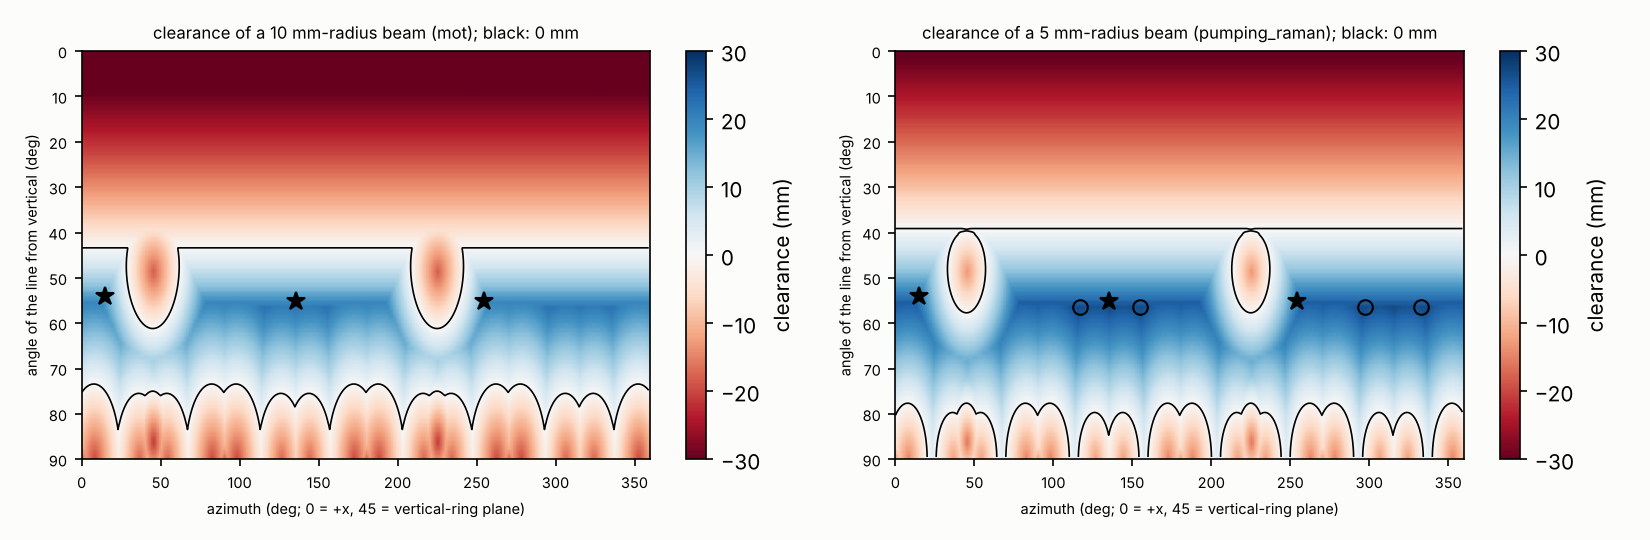
\includegraphics[width=\linewidth]{cavity_access/access.png}
\caption{Clearance of a beam through the atoms versus its direction (angle of the line from the
vertical; azimuth from $+x$; the vertical ring's plane is at \ang{45} and \ang{225}), for
\SI{20}{\milli\metre} (left) and \SI{10}{\milli\metre} (right) beams; black contour: zero clearance.
Each line through the atoms appears once (upper hemisphere). Stars: the three axes of the tilted six-beam
MOT; circles: the four pumping and Raman lines. Obstacles: all ring mirrors with a \SI{5}{\milli\metre} mount allowance and the
\SI{42}{\milli\metre} objective from \SI{38}{\milli\metre} above the atoms \placeholder{[CONFIRM?]}.}
\label{fig:access}
\end{figure}

\subsection{How many atoms loading needs}

A lattice site is $4\times4\times\SI{8}{\micro\metre\cubed} = \SI{1.3e-10}{\centi\metre\cubed}$. With the
usual collisional loading of about one atom in two sites \placeholder{[VALUE?: about 0.5 filling,
light-assisted collisions]}, each site of the loaded plane must first see about two atoms, i.e.\ a
density of about \SI{1.6e10}{\per\centi\metre\cubed} across the \SI{4}{\milli\metre} array. A MOT cloud
that keeps this density at the array corners (\SI{2.83}{\milli\metre}) with a peak three to five times
higher holds about $5\times10^{9}$ atoms, because most of its atoms lie in other planes. Accumulating
atoms in the in-plane sheets first, which span about 19 of the \SI{8}{\micro\metre} planes, reduces the
need to about $4\times10^{7}$ atoms delivered into the sheets, i.e.\ a MOT of $10^{8}$ to $10^{9}$ atoms
of at least \SI{6}{\milli\metre} extent. Demonstrated Cs numbers are $1.1(1)\times10^{9}$ atoms captured
in an optical molasses from a source of about $10^{10}$ atoms per second~\cite{DonleyNIST}, and
two-dimensional MOT fluxes of $4.02\times10^{10}$ atoms per second~\cite{Huang2016}. A tilted six-beam
MOT loaded from a two-dimensional MOT can therefore supply the atoms.

A single-beam grating MOT fits geometrically: a \SI{22}{\milli\metre} chip \SI{8}{\milli\metre} below
the atoms clears every ring beam by at least \SI{6.9}{\milli\metre}, its three \ang{45} diffracted beams
clear all mirrors and the objective by \SI{6.7}{\milli\metre}
\placeholder{[VALUE?: diffraction angle, set by the grating period]}, and the vertical axis below it is
free for \SI{96}{\milli\metre} (to G2) for a retro-reflector. Its single input beam must come from above,
along the objective axis. However, demonstrated grating MOTs are small for this purpose:
$2.46(7)\times10^{8}$ Rb atoms when loaded from a two-dimensional grating MOT~\cite{Imhof2017}, and for
Cs only $7.0\times10^{6}$ atoms, and only with an additional retro-reflected beam of \SI{69}{\percent}
of the input intensity; at \SI{24}{\percent} no atoms were trapped~\cite{Takamizawa2025}. A Cs grating MOT
is therefore one to two orders of magnitude short of a single-shot load of $10^{6}$ sites, and would need
iterative accumulation with the stored atoms shielded from the MOT light. We therefore recommend the
tilted six-beam MOT, with the grating MOT as a compact fallback for smaller arrays or with iterative
loading.

%======================================================================
\section{Noise and heating requirements}
\label{sec:noise}

We use the parametric-heating rates of Savard, O'Hara and Thomas~\cite{Savard1997}. Intensity noise
gives an energy e-folding time $T_I$ and position noise an energy-doubling time $T_x$,
\begin{equation}
  \frac{1}{T_I} = \pi^{2}\nu^{2} S_\epsilon(2\nu), \qquad
  \frac{1}{T_x} = \frac{\pi^{2}\nu^{2} S_x(\nu)}{\langle x^{2}\rangle}, \qquad
  \langle x^{2}\rangle = \frac{k_B T}{m (2\pi\nu)^{2}}.
  \label{eq:savard}
\end{equation}
Here, $\nu$ is the trap frequency in hertz, $S_\epsilon$ and $S_x$ are one-sided power spectral
densities of the fractional intensity and of the trap position, $m$ is the atomic mass and $T$ the
temperature. Our implementation reproduces their numerical examples ($3.2\times10^{-6}$\rtHz{} and
$3.2\times10^{-12}$\,m\rtHz{} for \SI{100}{\second} at \SI{10}{\kilo\hertz}). The position term is a
constant heating rate, $\dot E = 4\pi^{4} m \nu^{4} S_x$, independent of temperature. We quote it for
atoms at $T = \SI{10}{\micro\kelvin}$ \placeholder{[VALUE?: temperature after cooling in the lattice]},
so that a \SI{10}{\second} doubling time is \SI{1}{\micro\kelvin\per\second}, about one vibrational
quantum per second at \SI{20}{\kilo\hertz}.

The site shift of the self-intersecting ring is $a\,\mathrm{d}\phi/(2\pi)$, where $\mathrm{d}\phi$ is the
change of the phase accumulated between the two passes through the crossing, over the path
$L_1 = L_\mathrm{rt}/2$. This gives four couplings. (i) A normal displacement $d$ of one ring mirror at
incidence AOI, with the laser locked to the round trip $L_\mathrm{rt}$, shifts the sites by
$a\,(2 d \cos\mathrm{AOI}/\lambda)(1 - L_1/L_\mathrm{rt})$, i.e.\ by $3.2\,d$ for the in-plane rings and
$6.4\,d$ for the vertical ring at \ang{30}. (ii) A laser frequency change $\mathrm{d}\nu$ that the lock
does not remove shifts them by $a L_1\,\mathrm{d}\nu/c$ ($7.7\times10^{-15}$ and
$2.2\times10^{-14}$\,m/Hz). (iii) A change $\mathrm{d}\theta$ of the crossing half-angle changes the pitch
by $a\cot\theta\,\mathrm{d}\theta$ and moves the edge sites by $(S/2)\cot\theta\,\mathrm{d}\theta$
(\SI{14.7}{\milli\metre\per\radian}, in-plane). For the vertical lattice the array is perpendicular to the
lattice vector, so a symmetric angle change only rescales the period about the loaded plane at the
crossing; a single-arm change tilts the planes by $\mathrm{d}\theta/2$ and moves the edge sites by
$S\,\mathrm{d}\theta/(2\sqrt{2})$ (\SI{1.41}{\milli\metre\per\radian}; an estimate). (iv) A residual laser-cavity detuning $\mathrm{d}\nu_r$ modulates
the circulating intensity by $-(2\,\mathrm{d}\nu_r/\kappa_c)^{2}$, where $\kappa_c$ is the full linewidth.
For Gaussian $\mathrm{d}\nu_r$ with a flat one-sided spectrum $S_\nu$ over a bandwidth
$B = \SI{100}{\kilo\hertz}$ this gives
\begin{equation}
  S_\epsilon \approx \frac{32 S_\nu^{2} B}{\kappa_c^{4}}, \qquad
  S_\epsilon = \frac{64\,\delta_0^{2} S_\nu}{\kappa_c^{4}}\ \text{(linear term, static offset $\delta_0$)}.
  \label{eq:lock}
\end{equation}
The linewidths are those of the over-coupled design point with the 258 and \SI{181}{\mega\hertz} free
spectral ranges. Table~\ref{tab:noise} gives the requirements.

\begin{table}[htbp]
\centering
\caption{Noise requirements as one-sided amplitude spectral densities: position, displacement, frequency
and angle at $\nu$; intensity at $2\nu$; lock residual flat over \SI{100}{\kilo\hertz}, zero offset. Atoms
at \SI{10}{\micro\kelvin}; one mirror at \ang{30} incidence.}
\label{tab:noise}
\setlength{\tabcolsep}{3pt}
\begin{tabularx}{\linewidth}{@{}>{\raggedright\arraybackslash}p{1.8cm}>{\centering\arraybackslash}X>{\centering\arraybackslash}X>{\centering\arraybackslash}X>{\centering\arraybackslash}X>{\centering\arraybackslash}X>{\centering\arraybackslash}X>{\centering\arraybackslash}X>{\centering\arraybackslash}p{1.8cm}@{}}
\toprule
\hspace{0pt}Lattice, depth & \hspace{0pt}$\nu$ (\si{\kilo\hertz}) & \hspace{0pt}Heating time & \hspace{0pt}RIN at $2\nu$ (\si{\dBc\per\hertz}) & \hspace{0pt}Site position (pm\rtHz) & \hspace{0pt}One mirror (pm\rtHz) & \hspace{0pt}Laser frequency (Hz\rtHz) & \hspace{0pt}Crossing angle, edge (nrad\rtHz) & \hspace{0pt}Lock residual $G = 300$ / 1500 (Hz\rtHz) \\
\midrule
In-plane, \SI{0.2}{\milli\kelvin} & 19.8 & \SI{10}{\second} & $-106$ & 1.0 & 0.32 & 132 & 0.070 & 22 / 4.4 (7.0 / 1.4 kHz rms) \\
In-plane, \SI{0.2}{\milli\kelvin} & 19.8 & \SI{100}{\second} & $-116$ & 0.32 & 0.10 & 42 & 0.022 & 12 / 2.5 \\
In-plane, \SI{0.86}{\milli\kelvin} & 41.0 & \SI{10}{\second} & $-112$ & 0.24 & 0.074 & 31 & 0.016 & 15 / 3.0 \\
Vertical, \SI{0.2}{\milli\kelvin} & 9.9 & \SI{10}{\second} & $-100$ & 4.1 & 0.64 & 186 & 2.9 & 22 / 4.3 \\
Vertical, \SI{0.86}{\milli\kelvin} & 20.5 & \SI{10}{\second} & $-106$ & 0.95 & 0.15 & 43 & 0.68 & 15 / 3.0 \\
\bottomrule
\end{tabularx}
\end{table}

Seven conclusions follow. (i) The cavity passes the laser's relative intensity noise unchanged below
$\kappa_c/2$ (\SI{206}{\kilo\hertz} at $G = 300$), so the input beam itself needs \SI{-106}{\dBc\per\hertz}
at \SI{40}{\kilo\hertz} for \SI{10}{\second} at \SI{0.2}{\milli\kelvin}, and \SI{-116}{\dBc\per\hertz} for
\SI{100}{\second}. This is a requirement on the amplifier and the intensity servo, not on the cavity
\placeholder{[VALUE?: RIN of a stabilised 1075 nm fibre amplifier at 20 to 80 kHz]}. (ii) The residual
detuning must stay below \SI{22}{\hertz}\rtHz{} over \SI{100}{\kilo\hertz} (\SI{7.0}{\kilo\hertz} rms,
\SI{1.7}{\percent} of the \SI{413}{\kilo\hertz} linewidth) at $G = 300$, and below \SI{4.4}{\hertz}\rtHz{}
(\SI{1.4}{\kilo\hertz} rms) at $G = 1500$. The requirement scales as $\kappa_c^{2}$ in the quadratic
regime, so $G = 1500$ is five times harder; a static offset of \SI{1}{\percent} of the linewidth makes
the linear conversion comparable (26 and \SI{5.2}{\hertz}\rtHz). This quantifies the reason for working at
$G \approx 300$. (iii) Position noise is the stricter condition. A site motion of \SI{1}{\pico\metre}\rtHz{}
at \SI{20}{\kilo\hertz}, one quantum per second, corresponds to a single-mirror displacement of
\SI{0.32}{\pico\metre}\rtHz, or \SI{0.1}{\pico\metre}\rtHz{} for \SI{100}{\second}. Coating Brownian
noise is far below this \placeholder{[VALUE?: approx. 1e-17 m/rtHz at kHz, verify]}; the relevant
source is the excitation of mount and spacer resonances in the 10 to \SI{40}{\kilo\hertz} band by
acoustic noise, pumps and the lock actuator. Hence the ring should be a monolithic, low-expansion
assembly, as in Ref.~\cite{Park2022}, with its lowest mechanical resonances either above about
\SI{50}{\kilo\hertz} or well damped \placeholder{[VALUE?: mount vibration spectrum]}. (iv) With the laser
locked to the ring, its frequency follows the round-trip length, and coupling (i) already includes this
through the factor $(1 - L_1/L_\mathrm{rt})$; the laser-frequency column applies to noise that the lock
does not remove, i.e.\ above the lock bandwidth and below $\kappa_c/2$, and a lock bandwidth above $2\nu$
avoids it. (v) Edge sites move by \SI{14.7}{\milli\metre} per radian of crossing-angle change, so
\SI{0.07}{\nano\radian}\rtHz{} is needed at \SI{20}{\kilo\hertz}; for a mirror mount with a
\SI{10}{\milli\metre} lever this is \SI{0.7}{\pico\metre} of differential motion, comparable to (iii)
and not a separate technology. For the vertical lattice the corrected lever relaxes this to
\SI{2.9}{\nano\radian}\rtHz{} at \SI{10}{\kilo\hertz}. (vi) The cavity is a mode filter for input pointing jitter. The nearest
transverse mode of the \SI{70}{\milli\metre} ring lies \SI{0.216}{\radian} from the fundamental per round
trip, i.e.\ \SI{8.9}{\mega\hertz}, against a \SI{206}{\kilo\hertz} half-linewidth at $G = 300$; input
misalignment therefore couples into it with about 0.02 of the amplitude it would have without the
cavity, and the site positions are set by the mirrors, not by the input beam. (vii) The vertical
lattice, with its lower trap frequency at \SI{0.2}{\milli\kelvin}, is the least sensitive to intensity
noise (\SI{-100}{\dBc\per\hertz} at \SI{20}{\kilo\hertz}), but its larger lever gives a similar mirror
requirement (\SI{0.64}{\pico\metre}\rtHz).

These are requirements, not predictions: we have not simulated the time-dependent depth and site
position, nor estimated the vibration spectrum of a real mount.

%======================================================================
\section{How large a step is $10^{6}$ sites?}
\label{sec:scaling}

To see which constraints are specific to $10^{6}$ sites, we ran the same models at $10^{4}$
($100\times100$ sites, \SI{0.40}{\milli\metre} side) and $10^{5}$ ($316\times316$,
\SI{1.26}{\milli\metre} side), with the same pitch, barrier depth (\SI{0.2}{\milli\kelvin} per axis),
sheet thickness ($w_z = \SI{75}{\micro\metre}$), losses and $G = 300$. The runs comprise the Fox--Li
designs and spectra (depth rms converged to \SI{0.3}{\percent} of its value between 4096 and 16384
points), $\lambda/1000$ figure errors and \SI{1}{\micro\radian} tilts on every mirror with a
perfect-metrology redesign and the atom loop (correlation lengths scaled with the array side, so the
relative error structure is that of the 0.5 and \SI{2}{\milli\metre} cases at $10^{6}$), the vertical
ring and its mirror intensities. At each size we also ran the $10^{6}$ design unchanged.

The $10^{6}$ design does not scale down. Its telescope exists to break the degeneracy of a
\SI{5.5}{\milli\metre} flat mode, whose Fresnel number in the plain ring is 53. A smaller mode is
already non-degenerate, and the telescope then compresses it towards a focus on G. At $10^{4}$ the
telescope ring has an ideal non-uniformity of \SI{4.4}{\percent} at 0.73 of the enhancement and a
graded-mirror phase of \SI{1262}{\radian} peak to valley; $\lambda/1000$ errors give 9.9 and
\SI{23}{\percent}, and the atom loop fails (\SI{28.6}{\percent}, $G/G_0 = 0.09$). At $10^{5}$ the ideal is
\SI{0.31}{\percent} and errors give 6.6 and \SI{8.4}{\percent}. The vertical ring's $0.15\times$ telescope
fails in the same way (ideal \SI{9.8}{\percent} at $10^{5}$). The adopted design at $10^{4}$ and $10^{5}$
is therefore the plain ring, with plane folds and graded mirrors \SI{150}{\milli\metre} from the crossing,
for the in-plane and the vertical axes. Its mirrors must be larger than the $10^{6}$ strips in the
direction of the small flat-tops, which diffract. With the $10^{6}$ apertures (2.5 and
\SI{5}{\milli\metre} half-widths) the design target of the $10^{5}$ vertical ring loses $1.6\times10^{-3}$
and $2.0\times10^{-2}$ per round trip (enhancement 0.78); with 8 and \SI{15}{\milli\metre} it loses
$1.6\times10^{-8}$ and $3.4\times10^{-5}$. Table~\ref{tab:scaling} and Fig.~\ref{fig:scaling} compare the three sizes.

\begin{table}[htbp]
\centering
\caption{The cavity lattice at three array sizes, \SI{0.2}{\milli\kelvin} barrier per axis, $G = 300$.
Two values separated by a comma are two random error realisations; h and v denote errors in the
horizontal and vertical direction of the vertical ring.}
\label{tab:scaling}
\begin{tabularx}{\linewidth}{@{}>{\raggedright\arraybackslash}p{4.3cm}>{\raggedright\arraybackslash}X>{\raggedright\arraybackslash}X>{\raggedright\arraybackslash}X@{}}
\toprule
 & $10^{4}$ sites & $10^{5}$ sites & $10^{6}$ sites \\
\midrule
Array side; in-plane flat-top equivalent width & 0.40; \SI{0.55}{\milli\metre} & 1.26; \SI{1.74}{\milli\metre} & 4.00; \SI{5.51}{\milli\metre} \\
Hologram tweezers, input & \SI{14}{\watt} & \SI{140}{\watt} & \SI{1399}{\watt} \\
Lattice in free space, input & \SI{69}{\watt} & \SI{150}{\watt} & \SI{1041}{\watt} \\
Cavity lattice, input at $G = 300$ / 1500 & 0.23 / \SI{0.046}{\watt} & 0.50 / \SI{0.10}{\watt} & 3.5 / \SI{0.69}{\watt} \\
Tweezer power over cavity input ($G = 300$) & 61 & 279 & 403 \\
Vertical ring share of circulating power & \SI{69}{\percent} & \SI{55}{\percent} & \SI{79}{\percent} \\
Adopted vertical ring & plain, Gaussian vertical profile ($w = \SI{266}{\micro\metre}$) & plain, order-10 vertical flat-top & $0.15\times$ horizontal, $4\times$ vertical telescope \\
Adopted in-plane ring & plain, $p = \SI{150}{\milli\metre}$ & plain, $p = \SI{150}{\milli\metre}$ & $0.2\times$ telescope \\
Plain ring: Fresnel number; nearest mode (phase, loss) & 0.52; \SI{0.78}{\radian}, $2.4\times10^{-2}$ & 5.3; \SI{0.17}{\radian}, $2.5\times10^{-4}$ & 53; \SI{0.017}{\radian}, $2\times10^{-9}$ \\
Ideal non-uniformity, in-plane & \SI{0.059}{\percent} & \SI{0.053}{\percent} & \SI{0.23}{\percent} \\
$\lambda/1000$ on every mirror: uncorrected; perfect redesign; atom loop & 2.0, 3.0\%; 1.3, 0.77\%; 3.0, 2.8\% & 1.6, 2.6\%; 0.16, 0.17\%; 0.20, 0.49\% & 2.0, 4.0\%; 0.41, 0.49\%; 0.42, 0.75\% \\
The same, \SI{0.5}{\milli\metre}-scale errors (scaled) & 4.2\%; 2.4\%; 5.8\% & 6.6\%; 2.2\%; 2.0\% & 3.6\%; 2.4\%; 2.3\% (\SI{50}{\milli\metre} ring) \\
\SI{1}{\micro\radian} tilts on every mirror, uncorrected & 0.08, 0.10\% & 1.1, 0.19\% & 1.1\% \\
Plain ring at this size, $\lambda/1000$, uncorrected & 2.0, 3.0\% & 1.6, 2.6\% & 20, 42\% \\
Hottest in-plane mirror & \SI{4.2}{\kilo\watt\per\centi\metre\squared} (fold) & \SI{4.2}{\kilo\watt\per\centi\metre\squared} (fold) & \SI{48}{\kilo\watt\per\centi\metre\squared} (P2) \\
Largest absorbing defect, in-plane, silica / sapphire & 1.6 / \SI{39}{\micro\metre} & 1.6 / \SI{39}{\micro\metre} & 0.14 / \SI{3.4}{\micro\metre} \\
Vertical ring: ideal; $\lambda/1000$ uncorrected; after atom loop & 0.24\%; 2.9, 3.4\% (h), 0.28, 0.24\% (v); 0.43\% (one run) & 0.20\%; 10, 12\% (h), 1.6, 4.1\% (v); 1.4\% (one run) & 0.073\%; 5.7, 12\% (h), 5.4, 7.3\% (v); 1.06, 0.96\% (best round) \\
Vertical ring, hottest mirror & \SI{25}{\kilo\watt\per\centi\metre\squared} (P1) & \SI{7.4}{\kilo\watt\per\centi\metre\squared} (P1) & \SI{55}{\kilo\watt\per\centi\metre\squared} (G, P2$'$) \\
Edge-site crossing-angle requirement, \SI{10}{\second} at \SI{10}{\micro\kelvin} & 0.70\,nrad\rtHz & 0.22\,nrad\rtHz & 0.070\,nrad\rtHz \\
MOT atoms needed: cloud matched at the corners; into the sheets & $4.7$ to $5.0\times10^{6}$; $3.7\times10^{5}$ & $1.5$ to $1.6\times10^{8}$; $3.7\times10^{6}$ & $4.8$ to $5.1\times10^{9}$; $3.7\times10^{7}$ \\
\bottomrule
\end{tabularx}
\end{table}

\begin{figure}[htbp]
\centering
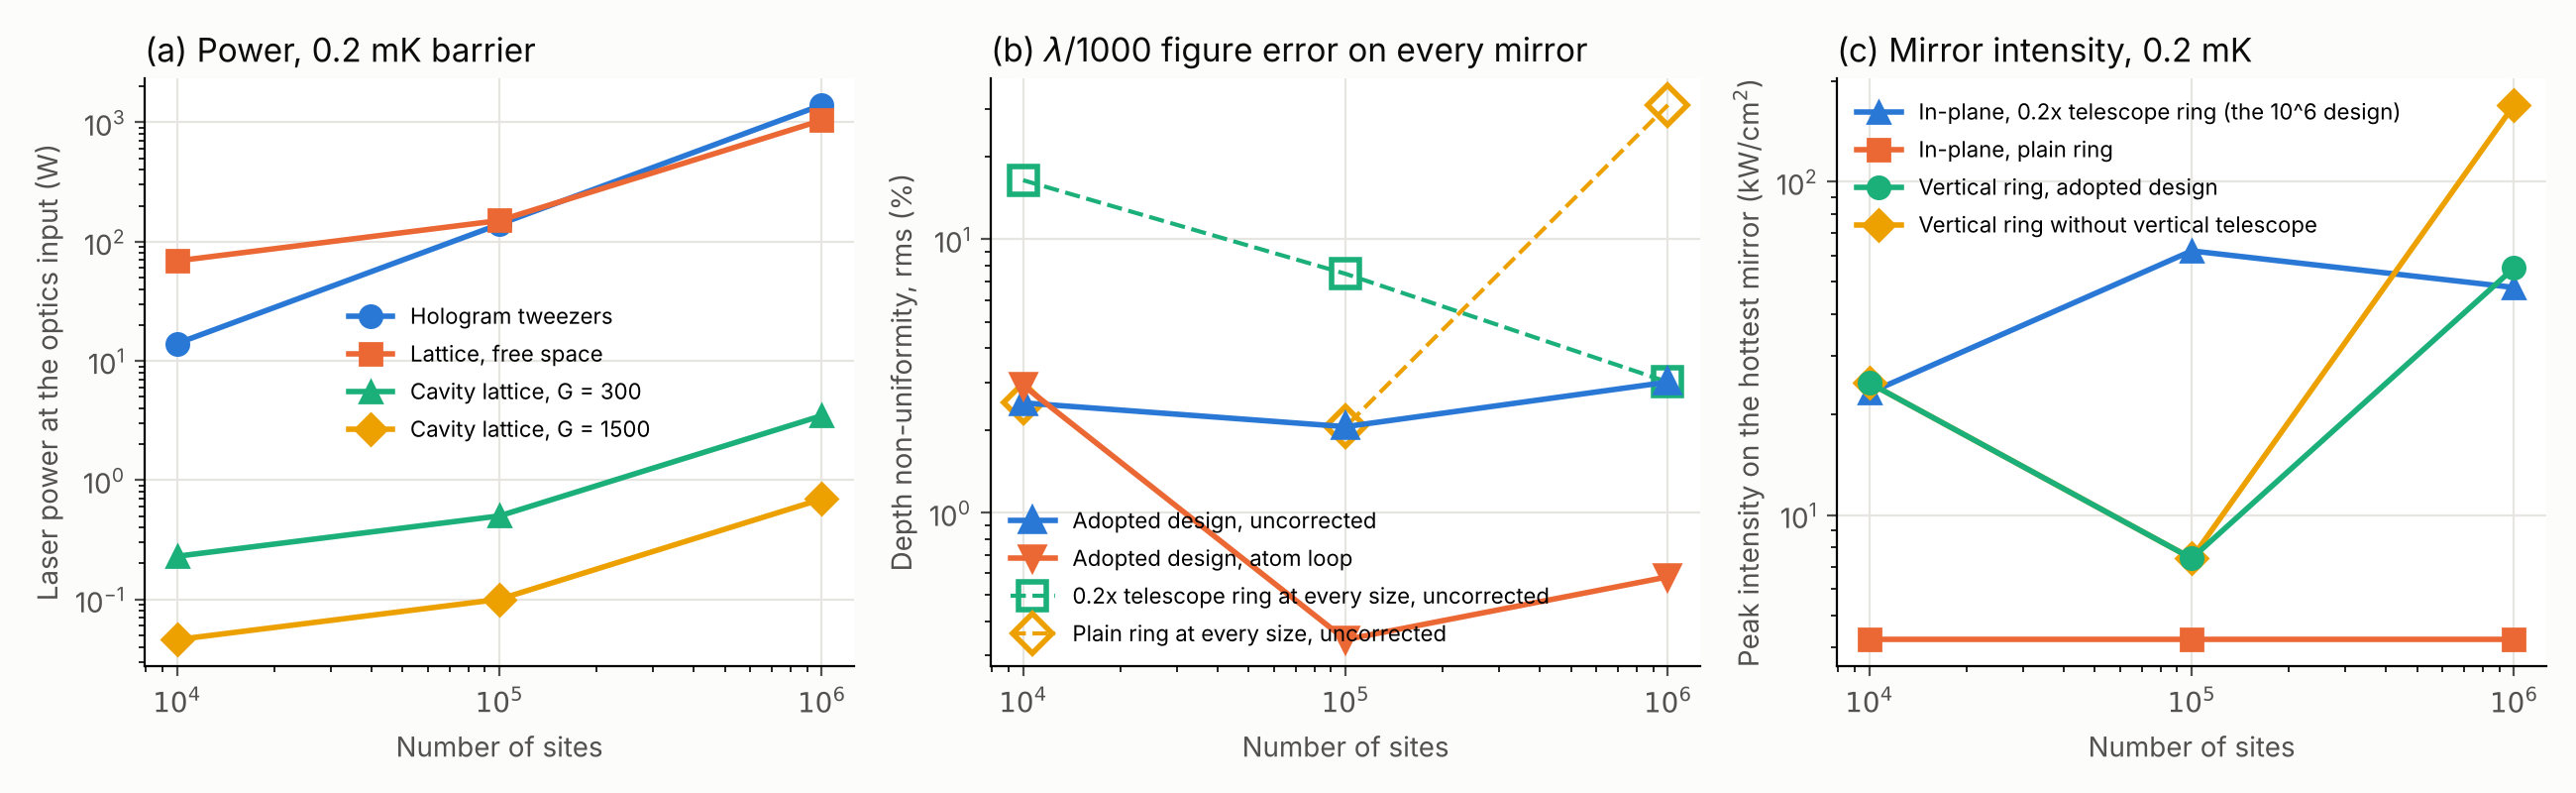
\includegraphics[width=\linewidth]{cavity_scaling/scaling.png}
\caption{The cavity lattice at $10^{4}$, $10^{5}$ and $10^{6}$ sites (\SI{0.2}{\milli\kelvin} barrier per
axis, \SI{4}{\micro\metre} pitch, \SI{1075}{\nano\metre}). (a) Laser power at the optics input; cavity
inputs for $T = 3L$ and mode matching 0.95. (b) Depth non-uniformity with independent $\lambda/1000$
figure errors on every mirror (median of two realisations): the adopted design at each size (plain ring
at $10^{4}$ and $10^{5}$, $0.2\times$ telescope ring at $10^{6}$), uncorrected and after six rounds of atom
feedback, and the two ring types at every size (dashed). (c) Peak intensity of the beam cross-section on
the hottest mirror. Fox--Li strip models, 8192 points, $G = 300$.}
\label{fig:scaling}
\end{figure}

Six results follow. (i) Laser power is not a constraint at $10^{4}$ (\SI{14}{\watt} of tweezers), and a
lattice in free space needs more than tweezers below about $10^{5}$, because its in-plane power scales as
the array side and the tweezer power as the number of sites. The cavity reduces the input 61, 279 and
403 times against tweezers. Thus the cavity is a convenience at $10^{4}$, a large saving at $10^{5}$
(\SI{0.50}{\watt} against \SI{140}{\watt}) and necessary at $10^{6}$. The vertical ring takes 55 and
\SI{79}{\percent} of the power at $10^{5}$ and $10^{6}$, because its vertical flat-top must cover a walk-off
that grows with the array side; at $10^{4}$ it takes \SI{69}{\percent}, because the adopted Gaussian profile
(item (iv)) is wider than a flat-top would be. A sheet thickness scaled as the square root of the side, which keeps the same \SI{1}{\percent}
roll-off per array length, would lower the inputs to \SI{0.18}{\watt} (with the adopted Gaussian vertical ring) and \SI{0.40}{\watt}
($w_z = 24$ and \SI{42}{\micro\metre}). (ii) The plain ring is non-degenerate at $10^{4}$ and $10^{5}$, so
no telescope is needed. The same $\lambda/1000$ errors that give 20 to \SI{42}{\percent} in the plain
$10^{6}$ ring give 1.6 to \SI{3.0}{\percent} at the smaller sizes, and tilts become nearly harmless. The
atom loop corrects $10^{5}$ to 0.20 to \SI{0.49}{\percent}, but not $10^{4}$ (2.8 to \SI{3.0}{\percent}),
where a perfect-metrology redesign still reaches 0.77 to \SI{1.3}{\percent}. A follow-up run shows two
causes. First, the 48-bin fit over 100 sites per side overfits: with 24 bins the loop reaches 1.1 and
\SI{2.2}{\percent} at its best round. Second, the phase-only floor is itself 0.77 to \SI{1.3}{\percent} at this
size, and the loop drifts above it after its best round (to 1.9 and \SI{4.2}{\percent} after six). A camera loop
on the transmitted beams behaves the same way (best 1.3 and \SI{1.9}{\percent}, then drifting to 2.1 and
\SI{2.2}{\percent}). Correction at $10^{4}$ is therefore limited to about \SI{1}{\percent} by the phase-only
graded mirrors, and the loop needs a stopping rule. (iii) The intensity at the atoms is set by the depth, so it is the same at every size.
Without the telescope the in-plane mirrors see at most \SI{4.2}{\kilo\watt\per\centi\metre\squared}, and the
defect limit is \SI{1.6}{\micro\metre} on fused silica at $10^{4}$ and $10^{5}$, against
\SI{0.14}{\micro\metre} at $10^{6}$ (P2 of the telescope ring, \SI{48}{\kilo\watt\per\centi\metre\squared}). The $10^{5}$ vertical ring needs no vertical telescope: its hottest mirror
sees \SI{7.4}{\kilo\watt\per\centi\metre\squared}, against \SI{55}{\kilo\watt\per\centi\metre\squared} at
$10^{6}$ with its vertical telescope (\SI{170}{\kilo\watt\per\centi\metre\squared} without). (iv) At $10^{4}$ the vertical flat-top is only \SI{19}{\micro\metre} high and diffracts
strongly over the \SI{414}{\milli\metre} half trip. Even with $\pm\SI{25}{\milli\metre}$ of mirror height in
the ring plane the ideal non-uniformity is \SI{3.2}{\percent}, and $\lambda/1000$ errors reduce the
enhancement to as little as 0.10. A Gaussian vertical profile is the better choice at this size, and we adopt it: a
\SI{266}{\micro\metre} waist keeps the intensity within \SI{1}{\percent} over the $\pm\SI{19}{\micro\metre}$
walk-off and has a \SI{207}{\milli\metre} Rayleigh range. Simulated, it gives \SI{0.24}{\percent} ideal
non-uniformity; vertical-direction $\lambda/1000$ errors are nearly harmless (0.24 and \SI{0.28}{\percent}),
horizontal ones give 2.9 and \SI{3.4}{\percent}, and atom feedback reaches \SI{0.43}{\percent} (one run). The
price is 5.9 times the vertical power, \SI{45}{\watt} circulating and \SI{0.23}{\watt} of total input at
$G = 300$; its hottest mirror sees \SI{25}{\kilo\watt\per\centi\metre\squared}.
(v) Only the crossing-angle requirement depends on size; the intensity, lock and mirror requirements of
Section~\ref{sec:noise} are the same, because the trap frequency is. (vi) A MOT of about
$5\times10^{6}$ atoms suffices for a single-shot load at $10^{4}$, which the demonstrated Cs grating MOT
reaches with an added retro-reflected beam~\cite{Takamizawa2025}; at $10^{5}$ a grating MOT suffices only
if the atoms are accumulated in the sheets, and at $10^{6}$ it does not.

Thus the large step is from $10^{5}$ to $10^{6}$. Up to $10^{5}$ the design is a plain ring with mirrors of
modest quality: \SI{0.5}{\watt} of input, $\lambda/1000$ errors at the per-cent level that the atom loop
corrects, micrometre-scale defect tolerance and no telescope. At $10^{6}$ the mode becomes degenerate,
which brings the telescope, the \SI{0.14}{\micro\metre} defect limit, a vertical ring that needs its own
vertical telescope and sapphire mirrors, a threefold tighter angle stability and a
$10^{9}$-atom MOT.

%======================================================================
\section{Discussion and conclusions}
\label{sec:discussion}

What is shown, within the one-dimensional scalar model and the parameters explored, is the
following. A cavity cannot give a static meta-optic tweezer array a tenfold power reduction
($G \le 3.2$). A three-ring lattice with graded-phase mirrors and intracavity telescopes supplies
$10^{6}$ Cs sites at \SI{0.2}{\milli\kelvin} with \SI{3.5}{\watt} of input at $G = 300$, a factor 300
below the same lattice in free space and 400 below hologram tweezers, with the depth uniform to
\SI{0.23}{\percent} rms by design. Mirror errors of $\lambda/1000$ give a few per cent, and closed-loop
re-shaping of the graded mirrors, from the atoms or from cameras on the transmitted light, removes most
of it with 0.8 to \SI{3.2}{\nano\metre} of stroke.

What is model-dependent is the following. Every Fox--Li result treats the horizontal and vertical
profiles as separable, except one two-dimensional check per question, and uses static perturbations
with one or two random realisations per case. The vertical ring is modelled as the product of two
one-dimensional modes. The noise analysis gives requirements from analytic heating rates, not a
time-dependent simulation. The layout is a first-order design without mounts, coils or the vacuum
envelope.

What is extrapolated is the following. The intensities of 4.5 to \SI{48}{\kilo\watt\per\centi\metre\squared}
in the in-plane rings, and 32 to \SI{55}{\kilo\watt\per\centi\metre\squared} in the vertical ring with its
$4\times$ vertical telescope (up to \SI{170}{\kilo\watt\per\centi\metre\squared} without it), are comparable to those
on the test masses of gravitational-wave detectors, where point absorbers limit the stored
power~\cite{Brooks2021}. Their consequence for a cold-atom apparatus, in which the mirrors sit close to
alkali vapour, has not been tested.

The main limitation is therefore no longer laser power or metasurface heating but the mirrors: figure
and alignment stability at the $\lambda/1000$ and \SI{1}{\micro\radian} level between corrections,
absorbing defects no larger than \SI{0.14}{\micro\metre} on the fused-silica mirrors of the in-plane
rings and \SI{3.0}{\micro\metre} on the sapphire mirrors of the vertical ring with its $4\times$
vertical telescope, and vibration below \SI{0.3}{\pico\metre}\rtHz{} at the trap frequency. The next steps
are (i) a model-based closed loop, with a stopping rule, for large starting errors and for the vertical
ring, whose loop drifts after its best round; (ii) a time-dependent simulation of depth and site position under laser
and lock noise, with a vibration model of the ring mounts; and (iii) the loading of a single plane of the vertical lattice from the
tilted MOT.

\bibliographystyle{unsrtnat}
\bibliography{references}

%======================================================================
\appendix

\section{Design summary}
\label{app:summary}

\begin{table}[htbp]
\centering
\caption{Parameters of the adopted design for $10^{6}$ sites at a \SI{0.2}{\milli\kelvin} barrier per
axis (\SI{1075}{\nano\metre}, Cs). Input powers per ring are $P_\mathrm{circ}/(0.95\,G)$.}
\label{tab:summary}
\begin{tabularx}{\linewidth}{@{}>{\raggedright\arraybackslash}p{4.2cm}>{\raggedright\arraybackslash}X>{\raggedright\arraybackslash}X@{}}
\toprule
Quantity & Each in-plane ring (two) & Vertical ring \\
\midrule
Lattice period, crossing angle $2\theta$ & \SI{4}{\micro\metre}, \ang{15.4} & \SI{8}{\micro\metre}, \ang{7.7} \\
Mode at the atoms & order-20 flat-top, \SI{5.51}{\milli\metre} equivalent width, times Gaussian sheet $w_z = \SI{75}{\micro\metre}$ & flat-top \SI{6.9}{\milli\metre} wide, times order-10 flat-top of \SI{0.19}{\milli\metre} half-height \\
Telescope per half trip & $0.2\times$ Keplerian, $f_1 = \SI{100}{\milli\metre}$, P1 at \SI{70}{\milli\metre}, $L = \SI{100}{\milli\metre}$ & $0.15\times$, $f_1 = \SI{160}{\milli\metre}$, P1 at \SI{110}{\milli\metre}, $L = \SI{120}{\milli\metre}$ \\
Round trip, free spectral range, reflections & \SI{1.16}{\metre}, \SI{258}{\mega\hertz}, 10 & \SI{1.66}{\metre}, \SI{181}{\mega\hertz}, 10 \\
Circulating power & \SI{102}{\watt} & \SI{785}{\watt} \\
Input power at $G = 300$ (mode matching 0.95) & \SI{0.36}{\watt} & \SI{2.75}{\watt} \\
Linewidth (FWHM) at $G = 300$ / 1500 & 413 / \SI{82}{\kilo\hertz} & 289 / \SI{58}{\kilo\hertz} \\
Peak intensity on the mirrors & 4.5 (P1), 48 (P2), 17.4 (G) \si{\kilo\watt\per\centi\metre\squared} & 32 to \SI{55}{\kilo\watt\per\centi\metre\squared} with the adopted $4\times$ vertical telescope \\
Vertical telescope; strip half-heights in the ring plane & none & $4\times$ Keplerian ($f_{1z} = \SI{36.8}{\milli\metre}$); $\pm\SI{2}{\milli\metre}$ on P1, P3, $\pm\SI{6}{\milli\metre}$ elsewhere; sapphire \\
Trap frequency along the lattice axis & \SI{19.8}{\kilo\hertz} & \SI{9.9}{\kilo\hertz} \\
Depth uniformity: design / $\lambda/1000$ errors / after atom feedback & 0.23 / 2.0 to 4.0 / 0.42 to 0.75\,\% & 0.073 / 5.4 to 12 / 0.96 to 1.06\,\% (best round) \\
Static figure and tilt before correction & $\lambda/1000$ rms, below \SI{1}{\micro\radian} & $\lambda/1000$ rms \\
Noise for a \SI{10}{\second} heating time at \SI{10}{\micro\kelvin} & RIN below \SI{-106}{\dBc\per\hertz} at \SI{40}{\kilo\hertz}; \SI{0.32}{\pico\metre}\rtHz{} per mirror at \SI{20}{\kilo\hertz} & RIN below \SI{-100}{\dBc\per\hertz} at \SI{20}{\kilo\hertz}; \SI{0.64}{\pico\metre}\rtHz{} per mirror at \SI{10}{\kilo\hertz} \\
\bottomrule
\end{tabularx}
\end{table}

The total circulating power is \SI{989}{\watt} and the total input \SI{3.5}{\watt} at $G = 300$
(\SI{0.69}{\watt} at $G = 1500$), against \SI{1.04}{\kilo\watt} for the same lattice in free space and
\SI{1.40}{\kilo\watt} for meta-hologram tweezers.

\section{Reproducibility}
\label{app:repro}

All results come from the scripts and configurations of the repository; each run writes a
\texttt{params.json} with its configuration, git state and package versions next to its results.
Table~\ref{tab:repro} lists them. Every script is run as
\texttt{python scripts/<name>.py configs/<name>.yaml}, except the table generator.

\begin{table}[htbp]
\centering
\caption{Scripts, configurations and results behind each section.}
\label{tab:repro}
\begin{tabularx}{\linewidth}{@{}>{\raggedright\arraybackslash}p{3.3cm}>{\raggedright\arraybackslash}X>{\raggedright\arraybackslash}X@{}}
\toprule
Section & Script and configuration & Results \\
\midrule
\ref{sec:tweezer}, \ref{sec:budget} & \texttt{cavity\_budget}, \texttt{cavity\_tweezer\_bounds} & \nolinkurl{results/cavity_budget/budget.json}, \nolinkurl{results/cavity_tweezer_bounds/bounds.json} \\
\ref{sec:architecture}, \ref{sec:access} & \texttt{cavity\_layout}, \texttt{cavity\_vertical\_layout}, \texttt{plot\_cavity\_sketch}, \texttt{cavity\_lattice} & \nolinkurl{results/cavity_layout/}, \nolinkurl{results/cavity_vertical_layout/}, \nolinkurl{results/cavity_lattice/lattice.json} \\
\ref{sec:foxli} & \texttt{cavity\_foxli}; tables by \texttt{cavity\_report\_tables.py latex docs/report/tables} & \nolinkurl{results/cavity_foxli/foxli.json} \\
\ref{sec:correction} & \texttt{cavity\_correction}, \texttt{cavity\_2d\_check}, \texttt{cavity\_vertical} (\texttt{cavity\_vertical\_chosen.yaml}) & \nolinkurl{results/cavity_correction/}, \nolinkurl{results/cavity_2d_check/}, \nolinkurl{results/cavity_vertical_chosen/} \\
\ref{sec:defects} & \texttt{cavity\_thermal}, \texttt{cavity\_vertical\_mirrors}, \texttt{cavity\_thermal\_foxli} & \nolinkurl{results/cavity_thermal/}, \nolinkurl{results/cavity_vertical_mirrors/}, \nolinkurl{results/cavity_thermal_foxli/} \\
\ref{sec:access} (access) & \texttt{cavity\_access} & \nolinkurl{results/cavity_access/access.json}, \texttt{access.png} \\
\ref{sec:noise} & \texttt{cavity\_noise} & \nolinkurl{results/cavity_noise/noise.json} \\
\ref{sec:scaling} & \texttt{cavity\_scaling}; \texttt{cavity\_foxli}, \texttt{cavity\_correction}, \texttt{cavity\_vertical}, \texttt{cavity\_vertical\_mirrors} with the \texttt{\_n1e4}, \texttt{\_n1e5} and \texttt{\_plain\_n1e*} configurations & \nolinkurl{results/cavity_scaling/scaling.json} and the \nolinkurl{_n1e4}, \nolinkurl{_n1e5} result folders \\
\bottomrule
\end{tabularx}
\end{table}

The core model is in \texttt{src/metatrap/cavity/} (\texttt{budget.py}, \texttt{lattice.py},
\texttt{foxli.py}) and is tested by \texttt{tests/test\_cavity.py}.

\section{Provenance and open placeholders}
\label{app:provenance}

Every number in this report is of one of four kinds. SIM values come from simulations executed for
this report and hold only within the simulated regime; they should be reviewed before submission.
DERIVED values are calculations from stated inputs, and SOURCE values are taken from the references
listed above, each of which was retrieved and read. The precedent values of Park et al., Norcia et al.,
LIGO, Zeiss, the Cs MOT and grating-MOT experiments, and the heating rates of Savard et al.\ are SOURCE;
the cesium polarisability is the repository's implementation of Steck's data (DERIVED from a source not
re-read for this report); the tweezer anchors of 143 and \SI{80}{\milli\kelvin} site per watt are SIM
from earlier studies of this project; all Fox--Li, correction, two-dimensional, vertical-ring,
deformation and access results are SIM; the budget, layout, trap frequencies, loading estimate and noise
requirements are DERIVED. The full ledger, with one row per value and its file pointer, is in the
working edition (\texttt{docs/cavity\_concept.md}, Verification notes).

{\raggedright The open placeholders, as marked in the working edition, are: \placeholder{[VALUE?: AR loss per surface 2.5e-4 to 1e-3]}; \placeholder{[VALUE?: Brewster residual loss 1e-4]}; \placeholder{[VALUE?: IBS absorption 1 ppm]}; \placeholder{[VALUE?: refractive objective 0.95, ideal relay 0.995 per pass]}; \placeholder{[VALUE?: mode-converter coupling 0.95]}; \placeholder{[CONFIRM?: cell wall 15 mm from the atoms; cell size for the layout]}; \placeholder{[REF?: freeform figuring at nm rms over mm apertures]}; \placeholder{[VALUE?: absolute flat-calibration agreement approx. 0.4 nm]}; \placeholder{[VALUE?: loss and stability of an intracavity deformable mirror]}; \placeholder{[CONFIRM?: objective position and mount, chamber windows, mounts]}; \placeholder{[VALUE?: grating diffraction angle]}; \placeholder{[VALUE?: about 0.5 collisional filling]}; \placeholder{[VALUE?: atom temperature 10 uK in the lattice]}; \placeholder{[VALUE?: RIN of a stabilised 1075 nm fibre amplifier]}; \placeholder{[VALUE?: coating Brownian noise approx. 1e-17 m/\rtHz{}]}; \placeholder{[VALUE?: mount vibration spectrum at 10 to 40 kHz]}; \placeholder{[VALUE?: tolerable vertical depth non-uniformity]}; \placeholder{[VALUE?: expansion coefficients of ULE, Invar, stainless steel, aluminium]}; \placeholder{[VALUE?: emissivity 0.9]}; \placeholder{[VALUE?: absorption of a figured graded mirror]}; \placeholder{[VALUE?: vibration of a water-cooled mount]}; \placeholder{[VALUE?: MOT coil dissipation]}; \placeholder{[VALUE?: amplifier cooling]}.\par}

\end{document}
